% !TEX root = main.tex
\documentclass[12pt,a4paper]{article}


% Encoding and language
\usepackage[utf8]{inputenc}
\usepackage[T1]{fontenc}
\usepackage[british]{babel}
\usepackage{csquotes} % Required for biblatex with APA style

% Margins and spacing
\usepackage[a4paper, top=2cm, bottom=2cm, left=2.5cm, right=2.5cm]{geometry}
\usepackage{setspace}
\onehalfspacing
\usepackage{makecell}
\usepackage{pdflscape}

% Bibliography with APA style (only biblatex)
\usepackage[style=apa, backend=biber]{biblatex}
\addbibresource{references.bib}
\DeclareLanguageMapping{british}{british-apa}

% Maths
\usepackage{amsmath, amsfonts, mathrsfs}

% Tables and figures
\usepackage{booktabs, threeparttable, caption, float, adjustbox, rotating, colortbl, diagbox}
\captionsetup[table]{position=top}
\usepackage{subcaption}
\usepackage{tabularray}

% Algorithms and code
\usepackage{algorithm}
\usepackage{algpseudocode}
\usepackage{listings}

% Graphics and plots
\usepackage{graphicx, tikz}
\usetikzlibrary{arrows.meta, positioning}
\usepackage{pgfplots}
\pgfplotsset{compat=1.18}

% Other utilities
\usepackage{authblk}
\usepackage{enumitem}
\usepackage{titlesec}
\usepackage{hyperref}
\hypersetup{colorlinks=true, allcolors=blue}
\usepackage{lineno}
\renewcommand\linenumberfont{\normalfont\scriptsize\sffamily\color{blue}}
\rightlinenumbers
% \linenumbers % Uncomment to enable line numbers

% Optional: custom subsection style
\titleformat{\section}{\normalfont\Large\bfseries}{\thesection.}{1em}{}

% Custom fourth-level section
\newcommand{\subsubsubsection}[1]{%
  \vspace{\baselineskip}%
  \noindent\textbf{#1\\}\quad%
}

% Unnumbered list
\makeatletter
\newenvironment{unlist}{%
  \begin{list}{}{%
    \setlength{\labelwidth}{0pt}%
    \setlength{\labelsep}{0pt}%
    \setlength{\leftmargin}{2em}%
    \setlength{\itemindent}{-2em}%
    \setlength{\topsep}{\medskipamount}%
    \setlength{\itemsep}{3pt}%
  }%
}{%
  \end{list}%
}
\makeatother



%-------------------------------------------
% Paper Head
%-------------------------------------------
\title{On the dark Paths of Populism: Can state Policy Reduce Electoral Support for Populism? Evidence from France}

\author{
  Yannay Spitzer\thanks{yannay.spitzer@mail.huji.ac.il} \and 
  Ilan Pargamin\thanks{ilan.pargamin@mail.huji.ac.il}
}
\affil{\small Hebrew University of Jerusalem}

\date{August 2024} 

\begin{document}

\maketitle

\begin{abstract}


We show the effectiveness of a spatial redistribution program in reducing electoral support for populism, using evidence from a tax credit program targeted at rural areas in France. The Zone de Revitalization Rurale (ZRR) program, launched in 1995, aimed to promote economic development and employment in rural areas through various corporate and payroll tax exemptions. Employing a spatial regression discontinuity design, we compare small rural municipalities situated near the ZRR program boundary. My findings reveal that municipalities benefiting from the ZRR program experienced a 0.3-0.5 percentage point reduction in National Front (FN) vote share in the 2002 presidential election, translating to a 3-5\% decrease on average relative to an average vote of 17\%. We argue that while the ZRR program was neither explicitly designed to counter populism nor effective in improving local economic conditions, the perceived support from the central state helped alleviate social discontent and reduce populist voting. This paper contributes to the growing literature on the socioeconomic and demographic determinants of populism by providing causal evidence of the role of geographic-based redistribution policies. 


\end{abstract}

\textbf{Keywords}: Populism, Inequalities, Redistribution, Policy, France rurality, RDD.  
\newpage


\small{
\textit{Passing through these villages felt like reviewing the façades in mourning. What wasn't closed was for sale, and what was for sale found no buyers. The war memorials bore glorious names, and it seemed to us that the few living souls wandering the streets could have been added to the list. [...] We were in the heart of the lost country, in the gray areas of "hyper-rurality." The inhabitants of this desert convinced themselves that Paris could not hear them.}\footnote{Original text translated by the author: \textit{Traverser ces villages donnait l'impression de passer la revue des façades en berne. Ce qui n'était pas fermé était à vendre, ce qui était à vendre ne trouvait pas acquéreur. Les monuments aux morts portaient les noms glorieux et il nous semblait que les quelques vivants vaquant dans les rues auraient pu s'ajouter à la liste. […] Nous étions là au cœur du pays perdu, dans les zones grises de « l'hyper ruralité ». Les habitants de ce désert se persuadaient que Paris ne les entendait pas.}}

		Sylvain Tesson, \textit{Sur les chemins noirs} (On the dark Paths), Gallimard, 2016, p. 82}



%-------------------------------------------
% Paper Body
%-------------------------------------------

\section{Introduction}

% Motivation
Can state policies reduce support for populism? The causes of populist voting have garnered significant interest in the scientific community (\cite{Guriev2022}). However, few studies have explored whether state policies can mitigate the rise of populism and directly address the underlying causes of social discontent.

This literature suggests that feelings of being "left behind" economically, culturally, or geographically, may play a central role in the surge of populist support. When individuals perceive that they have been excluded from the benefits of globalization or national prosperity, they may become more susceptible to anti-establishment and populist appeals.

I propose to evaluate the effect of a French Enterprise-Zone (EZ) on voting for the main right populist party, the FN. The ZRR (Zone de Revitalization Rurale) aimed to promote economic development, boost employment, and encourage population retention and attraction in low-density rural areas in France. The ZRR program, officially launched in September 1996, covered about 39\% of the French territory but only around 8\% of the population. The budgetary cost between 1995 and 2005 (first phase of the program) was approximately of 100 million euros and 400 million euros after 2005 (second phase). Although the ZRR program was not specifically designed to counter populism, it may influence populist voting through two potential mechanism. First, such a redistribution policy might enhance the socioeconomic and sociodemographic conditions of its recipients, thereby reducing social distress and discontent. Second, these transfers could reduce feelings of alienation and frustration among local communities toward the central state by affirming that they, too, share in the benefits of national growth. In turn, this may help to reduce populist sentiments in electoral outcomes.




The causal channels can be summarized as follows:
\vspace{0.5cm}

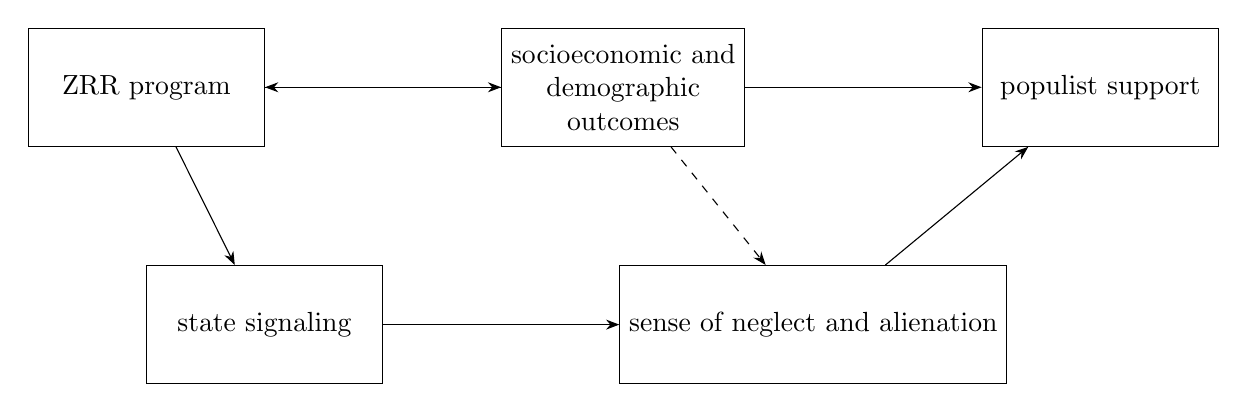
\begin{tikzpicture}[
  node distance=2cm and 3cm,
  every node/.style={draw, align=center, minimum width=3cm, minimum height=1.5cm},
  arrow/.style={-{Stealth}}
]

% Nodes
\node (zrr) {ZRR program};
\node (socio) [right=of zrr] {socioeconomic and \\ demographic \\ outcomes};
\node (populist) [right=of socio] {populist support};

\node (state) [below=1.5cm of zrr, xshift=1.5cm] {state signaling};
\node (isolation) [right=of state] {sense of neglect and alienation};

% Arrows
\draw [arrow] (zrr) -- (socio);
\draw [arrow] (socio) -- (zrr);
\draw [arrow] (socio) -- (populist);
\draw [arrow, dashed] (socio) -- (isolation);
\draw [arrow] (zrr) -- (state);
\draw [arrow] (state) -- (isolation);
\draw [arrow] (isolation) -- (populist);

\end{tikzpicture}

The main obstacle to a clean identification of a causal effect of the ZRR program is that socioeconomic and demographic variables both influence the electoral behavior and the eligibility of the municipalities to the ZRR program. 

I overcome this challenge by employing several complementary empirical strategies, the main one being a spatial regression discontinuity design (RDD). This approach leverages the fact that the program's criteria were applied at the county (\textit{canton}) and district (\textit{arrondissement}) levels, two administrative tiers above the municipal (\textit{commune}) level. Consequently, many small municipalities outside the program are in fact comparable to those within it. From 1990 to 2004, France had 4,055 counties with considerable population diversity, each containing an average of 9 municipalities and 14,723 inhabitants. In my baseline sample, which includes municipalities within a 10-kilometer radius of the program boundary, there were 1,833 counties, each with 8 municipalities and an average of 9,391 inhabitants.\footnote{See Table \ref{tab:summary_stats_combined}} My identification strategy relies on the assumption that, conditional on the demographic characteristics of the county that influenced its eligibility chances to the ZRR program, there should be no major differences between municipalities that are geographically close to each other but separated by the treatment frontier.

The main finding is that the ZRR program reduced electoral support for the National Front (FN) by 0.3-0.5 percentage points, which, given the average FN vote share of 17\% in my sample, represents a decrease of 3-5\%. This result is sensitive but remains robust across different sample selections. Notably, the effect holds when narrowing the sample from municipalities within a 40km radius of the program boundary to those within just 10km. Further restricting the sample to only the municipalities directly on the border yields similar estimates. Eventually, the results provide causal evidence that geographic-based distribution can mitigate populist support. 

Studying the mechanisms is challenging. I find no conclusive evidence that the ZRR had any effect on various socioeconomic outcomes. There are two possible explanations. First, the identification strategy may lack robustness, potentially insufficient in statistical power or affected by endogeneity, limiting its ability to detect a clear effect of the redistribution policy. Second, the ZRR may have been unsuccessful in improving the recipients' socioeconomic conditions, as shown in \cite{BEHAGHEL20151}, suggesting that the observed effect on the populist vote is not driven by the usual socioeconomic factors. How can we interpret this result, then? I propose the hypothesis of "state signaling" and provide some evidence. The ZRR program was seen as an attempt by the central state to reduce the socioeconomic isolation of rural areas and promote national equity. It was well-received by rural populations and their mayors. As I show below, when the parliament tried to reduce the program's size in 2013, rural mayors pressured to have it reinstated. This indicates that, although the economic impact of the program may have been limited, it was highly valued by elected officials and by rural populations. To the extent that feelings of alienation were a cause for populist voting, the central government inadvertently mitigated them by demonstrating that it cared for the treated counties, even if its efforts were ineffective. This state signaling effect could be the one that mitigates the populist support. 

% Contribution
This paper contributes to the rapidly expanding literature on the socioeconomic and demographic determinants of populism in Western countries. As noted by \cite{Inglehart2016}, it is challenging to disentangle economic causes (such as industrial decline, trade globalization, automation, the 2008-09 global financial crisis, and austerity) from cultural ones (such as reactions against cultural changes, social-status shifts, and immigration).\footnote{\cite{Inglehart2016}; \cite{Margalit2022}; \cite{Algan2017}; \cite{BACCINI_WEYMOUTH_2021}; \cite{Ferrara2023}; \cite{Colantone2018}; \cite{Autor2020}; \cite{Malgouyres}; \cite{Dippel2015} ; \cite{Fetzer2019}; and many more} However, in a context where these factors reinforce each other interactively (\cite{Gidron2017}), policies aimed at redistribution and reducing regional inequalities can address both causes simultaneously.

Globalization creates a clear political divide between those left behind in rural or deindustrialized areas and the "trailblazers" in dense, cosmopolitan, and globalized cities.\footnote{"Les premiers de cordée" (the trailblazers), phrase used by E. Macron in 2018.} \cite{Goodhart} distinguishes between the "somewheres," who are more conservative and rooted in their local communities, and the "anywheres," who are more liberal and geographically mobile. Although this distinction does not fully capture the complexity and diversity of attitudes towards globalization, it is clear that rising social discontent is unevenly distributed across territories. This grants the welfare state a crucial role in addressing globalization-linked inequalities (\cite{Samuelson}, \cite{Stiglitz}, \cite{NBERw22676}).

Firstly, austerity measures and public service closures are expected to increase support for populist parties. In the UK, \cite{Fetzer2019} showed that less austerity could have prevented Brexit, while \cite{Vries} argue that closures in the National Health Service increased support for populist right parties. Exploiting an Italian reform in 2010 that reduced access to local public services in municipalities with fewer than 5,000 residents, \cite{Cremaschi} show that public service deprivation plays a crucial role in the increasing support for far-right parties in small municipalities. Our paper also employs a Difference-in-Differences (DID) methodology to assess wether the ZRR program mitigated support for far-right parties. We further enhance the robustness of our findings by incorporating a spatial Regression Discontinuity Design (RDD) approach. Secondly, the main policy implication of the winner-loser analysis is that appropriate redistributive policies aimed at compensating the losers should mitigate electoral support for populist parties. Reducing inequalities between the "geo-social classes" (\cite{Piketty}) should reduce electoral polarization between these groups.\footnote{"What is called the geo-social class is a mix of classical social classes (wealth, property, etc.), but also the integration into a territorial and productive fabric. For the same wealth, for the same income, it is not the same to live in a metropolis or in a village. If you are a worker exposed to international competition living in towns and villages, you will have, for example, a perception of international economic integration and commercial competition that can, over time, make you very skeptical of the successive left and right governments that created the current Europe, leading you to vote for the FN (National Front) and RN (National Rally). According to us, this is not primarily an anti-immigrant vote but perhaps a vote expressing a feeling of abandonment on the economic front." (https://www.radiofrance.fr/franceinter/podcasts/grand-canal/grand-canal-du-mardi-19-septembre-2023-3850330, translated by the author)} 

Less evidence exists regarding the state's ability to reduce support for populist parties by allocating resources or attention to the periphery.

Evidence from Italy (\cite{ALBANESE2022}) showed that larger EU financing in the 2013 general election led to a drop in populism by about 9\% of the mean of the dependent variable. In the British context, \cite{Becker2017} found no correlation between EU Structural funds and the Leave share. Despite the apparent policy consensus emerging from this analysis, our understanding of the effectiveness of redistribution in mitigating populism remains quite limited. To my knowledge, the aforementioned papers are the only ones that provide causal evidence for the redistribution effect. 

This paper aims to fill this gap in the French context by looking at a rural-oriented development program. Beyond providing evidence from a different country, this study contributes in three key ways. First, it evaluates a large-scale, nationally funded redistribution program, which covered approximately 8\% of the French population, about 4.5 million people. Second, the ZRR program targets rural areas based on demographic and economic thresholds, providing a natural and spatially precise setting for causal inference. Third, the study leverages a combination of Difference-in-Differences and spatial RDD designs, allowing for high internal validity. Notably, the ZRR program is the largest redistribution initiative for which electoral impacts have been measured. Additionally, this paper provides precise estimates of the ZRR effect because of the large sample of municipalities I build (France has about 35,000 communes).

The remainder of the paper is structured as follows. Section \ref{background} describes the background details and the data. 
Section \ref{fn-growth} presents some stylized facts on the FN growth. Section \ref{RDD} illustrates my identification framework and presents the main results as well as the robustness tests. I discuss these results in section \ref{results}. Section \ref{conclusion} concludes.




\section{Background}\label{background}
\subsection{Background}

\subsubsection{Determinants of populist voting}

[IP: this subsection is redundant with what comes before - I think that the lit survey on the determinants of populist voting is what's already in the introduction. I don't think we need to repeat it here] 

Populism thrives on the interaction between long-term economic transformations and cultural backlash. Key economic drivers include trade globalization, automation, and deindustrialization, which have left many regions—particularly rural and peri-urban areas—economically vulnerable. In parallel, cultural and identity-based grievances, often reinforced by status anxiety and perceived marginalization, further catalyze populist support.

In the US and Europe, the collapse of industrial employment, rising inequality, and falling social mobility have been shown to predict populist voting patterns (\cite{Autor2020}; \cite{Dippel2015}; \cite{Colantone2018}). In France, for example, \cite{Malgouyres} and  \cite{Algan2017} document that regions more exposed to import competition or economic negative shocks are also those where far-right support has increased most markedly.

Cultural backlash is another key driver of populist voting. \cite{Inglehart2016} argue that the rise of populism reflects a reaction against the erosion of traditional cultural values, particularly among older, less-educated, and more socially conservative voters who feel threatened by rapid cultural change, immigration, multiculturalism, and gender equality. \cite{Gidron2017} further highlight the role of status anxiety, showing that individuals with declining subjective social status are significantly more likely to support populist parties. \cite{Algan2017} show that distrust in political institutions and interpersonal trust are strong predictors of populist support, while \cite{Giuliano2020} and \cite{Rodriguez2021} find that declining social capital in peripheral areas correlates with higher populist vote shares. 

The 2008–09 global financial crisis and subsequent austerity programs were catalyzers of the populist sentiment. Fiscal austerity in the UK boosted support for right-wing populist parties (\cite{Fetzer2019}; \cite{Vries}). While much of the literature has focused on the negative political consequences of state withdrawal, relatively few studies provide causal evidence on the effects of positive redistribution. The aforementioned papers are among the rare exceptions (\cite{ALBANESE2022}; \cite{Becker2017}).


\subsubsection{Front National (FN)}

The FN was established in 1972, emerging from the remnants of various extreme-right groups (some Waffen-SS, members of the OAS, neo-Nazis and Vichy's nostalgic).\footnote{Organisation de l'Armée Secrète, a terrorist group that fought to keep Algeria as French.} Jean-Marie Le Pen played a pivotal role in uniting various factions under a common nationalist and populist agenda. The party's rhetoric and provocative statements, particularly Le Pen's controversial remarks about the Holocaust, garnered substantial media attention and public debate. 

The National Front's electoral breakthrough began in the March 1982 cantonal elections, where candidates reached or exceeded 10\% of the vote in places like Grande-Synthe (13.3\%) and Dreux-Est (19.6\%). Its rise is often traced to the March 1983 municipal elections, notably when Jean-Marie Le Pen received 11.26\% in Paris and a coalition in Dreux earned 31\% in the first round. The National Front gained national prominence in the June 1984 European elections, securing 10.95\% of the vote and ten seats in the European Parliament, marking its "entry into politics." On March 16, 1986, with a new proportional voting system, the National Front won 35 seats in the National Assembly.

Initially, the FN promoted economic liberalism and anti-communism, reflecting the right-wing and nationalist sentiments of its founders.\footnote{Published in 1978, "Doctrine économique et sociale du Front National", by Pierre Gérard, "a kind of 'liberal-national' manifesto that 'revisits Poujadist ideas and praises economic freedoms,' according to \cite{igounet2014}, would serve as the party's reference on economic issues until 1990."} However, as globalization and economic changes affected its voter base, the FN shifted towards a more protectionist and welfare-oriented economic stance. P.-A. Taguieff described this transition as a move from "national-liberalism" to "national-populism".\footnote{Pierre-André Taguieff, sociologist and historian, is the director of research at the French National Centre for Scientific Research (CNRS) in an Institut d'études politiques de Paris laboratory, the Centre for Political Research (CEVIPOF)} It was marked by advocating for policies that protect French jobs and industries from foreign competition, criticizing the European Union's economic policies, and promoting social welfare programs framed as benefiting "native" French citizens over immigrants. Specifically after the fall of the Berlin Wall, the National Front underwent a shift that led it, in the words of Bruno Mégret, to choose the camp of "nationalism" over "globalism." In his 2002 presidential platform, Jean-Marie Le Pen declared, "It is imperative to regulate trade with a measured protectionism." Denouncing "ultra-free-trade," the National Front leader aimed to "restore economic borders to France (and, if possible, to Europe)."\footnote{The campaign slogan "1  million de chômeurs, c'est 1 million d'immigrés en trop" (A million unemployed is a million immigrants too many) summarizes the FN's "national populism".} Jean-Marie Le Pen added, "We are against the euro, which eliminates France's sovereignty in the economic domain." He added that France must regain "control of its currency and, therefore, control over its economic and financial policy." Eventually, the 2002 presidential election was a turning point for the FN. Jean-Marie Le Pen's surprise qualification for the second round of the election shocked France. He received 16.86\% of the vote, surpassing the Socialist candidate Lionel Jospin. Despite losing to Chirac in the runoff, this event marked the FN's arrival as a significant force in French politics. Marine Le Pen took over the leadership from her father in 2011. Under her leadership, the FN sought to soften its image, distancing itself from the overtly xenophobic and anti-Semitic rhetoric of the past. The re-branding included a name change to "Rassemblement National" (National Rally) in 2018.

Initially, the FN resonated with a poujadist electorate composed mainly of small urban traders and artisans, employed and generally educated.\footnote{"Poujadism", named after Pierre Poujade, was a far-right political and trade union movement in France that emerged in 1953 in the Lot and dissolved in 1958. It advocated for the protection of small business owners and artisans, who were seen as threatened by the post-war expansion of large retail chains, and criticized the inefficacy of parliamentary governance under the Fourth Republic. The movement, associated with the Union de défense des commerçants et artisans and its political arm, Union et fraternité française, used strong-arm tactics in demonstrations and engaged in combative protests. Often seen as a "small-bourgeois conservatism," the term "poujadism" has come to refer pejoratively to reactionary, corporatist political movements. Notably, Jean-Marie Le Pen, later the founder of the National Front, began his political career as a Poujadist deputy.} Over time, however, this base shifted, and the FN increasingly attracted those who felt "left behind."

The FN was widely considered a populist party during our period of interest (1995-2002). This classification stems from its rhetoric that pits "the people" against "the elites," its anti-establishment stance, and its appeal to nationalism and sovereignty.\footnote{The American Heritage Dictionary defines populism as "a political philosophy supporting the rights and power of the people in their struggle against the privileged elite."} The party consistently portrays itself as the defender of ordinary French citizens against corrupt elites, both within France and in the broader European context. Its populist approach is characterized by a strong emphasis on national identity, opposition to immigration, and a critique of globalization. 



Figure \ref{fig:fn_vote_share} shows the evolution of the FN vote share in the first rounds of the different presidential elections. The scores of Jean-Marie Le Pen are stable around 13\%, while they reach 23\% in 2022 with Marine Le Pen. Lately, the party rose to prominence during the 2024 European elections by winning the highest vote share among all French political parties, as well as in the 2022 and 2024 legislative elections, and the first rounds of the 2017 and 2022 presidential elections. 


% FN results presidential across time
\begin{figure}[h]
    \centering
    \caption{Evolution of FN Vote Share (1988-2022) - Presidential Elections in France}
    \label{fig:fn_vote_share}
    
    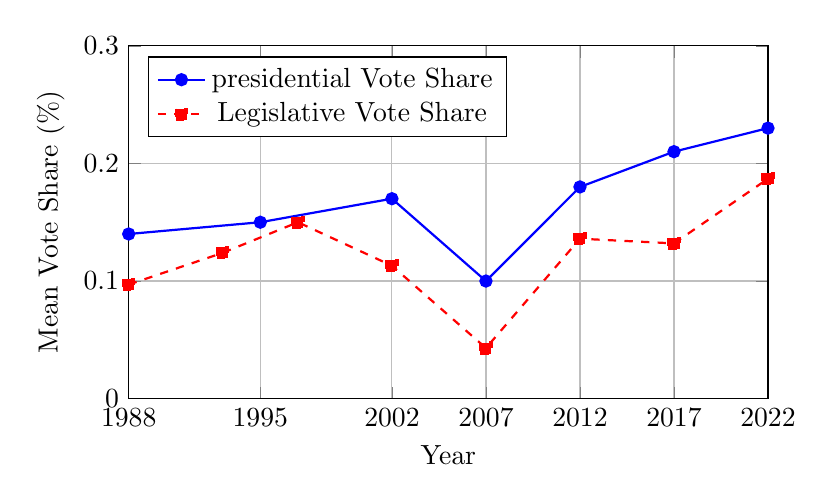
\begin{tikzpicture}
        \begin{axis}[
            width=0.8\textwidth,
            height=0.5\textwidth,
            xlabel={Year},
            ylabel={Mean Vote Share (\%)},
            ymin=0.0, ymax=0.3,
            xmin=1988, xmax=2022,
            xtick={1988, 1995, 2002, 2007, 2012, 2017, 2022},
            ytick={0.0, 0.1, 0.2, 0.3},
            grid=major,
            legend pos=north west,
            xlabel near ticks,
            ylabel near ticks,
            tick label style={/pgf/number format/1000 sep=}
        ]

        % Mean vote share
        \addplot[blue, mark=*, thick] table {
            1988 0.14
            1995 0.15
            2002 0.17
            2007 0.10
            2012 0.18
            2017 0.21
            2022 0.23
        };
        \addlegendentry{presidential Vote Share}
        
         % legislative
        \addplot[red, mark=square*, thick, dashed] table {
            1988 0.097
            1993 0.124
            1997 0.150
            2002 0.113
            2007 0.043
            2012 0.136
            2017 0.132
            2022 0.187
        };
        \addlegendentry{Legislative Vote Share}
        
        
        \end{axis}
    \end{tikzpicture}


\parbox{\textwidth}{\footnotesize \textit{Notes:} The vote shares correspond to the ratio of the number of votes Le Pen (Jean-Marie and, after 2011, Marine Le Pen) received to the total number of expressed votes in the first round of the presidential election.}
    

\end{figure}

\subsubsection{Socioeconomic evolution in rural France}

Non-urban communities are those that lagged behind economically and experienced slower growth in France over the past 30 years. They also are the ones where the electoral support for the FN increased the most in the same period. The literature identifies three main reasons to that differential increase: (i.) composition effect; (ii.) economic and social isolation; (iii.) state withdrawal.\footnote{There are additional and not necessarily contradictory explanations. The influential demographer Hervé Le Bras, in an interview to \textit{Le Monde} in 2022, explains the predominance of rural populist vote with the education-occupation gap: "One of the consequences of the remarkable increase in education levels and the number of graduates [...] is that the level of education individuals achieve no longer corresponds to the positions they occupy in society." In France, while 36\% of the working population have completed higher education, only 16\% are executives and professionals. This mismatch is more pronounced in rural areas: in municipalities with fewer than 1,000 inhabitants, 20\% of baccalaureate holders are white-collar workers, compared to 45\% in cities with more than 100,000 inhabitants."}

\begin{enumerate}
    \item \textbf{Composition effect}

This argument highlights the socio-demographic and economic changes France has experienced since the 1980s. Younger and more educated individuals have migrated to urban areas in search of better opportunities, leaving behind an older and less mobile population. \cite{Guilly2014} notes that the "forced" migration of the "native French" (those with both parents born in France) working class from urban to rural and deep suburban areas, mainly due to rising real estate prices, has created a divide.\footnote{The publication in 2014 of \textit{La France périphérique : Comment on a sacrifié les classes populaires} launched an intense debate in France. The concept "peripheral France" was criticized for its simplicity, but remains relevant in the French public discourse.} This divide separates them from recent immigrant suburbs on one side and the "globalized and gentrified" metropolitan areas on the other. This separation has fostered distrust towards both immigrants and globalized elites, leading to a cultural withdrawal into more socially and culturally homogeneous "hinterlands." Figure \ref{fig:FN_typology} displays the mean vote share for the Front National (FN) across three aggregated typologies—Rural, Intermediary, and Urban—calculated for the years 1988, 1995, 2002, and 2007. The FN vote increased relatively more in rural and intermediary municipalities than in urban ones. Similarly, support for the FN was initially strong among the top-income voters, but has since diminished, whereas support from lower-income deciles has increased. \footnote{\cite{Piketty}, Graph 12.19. While the top-income voters (top 5\% and top 1\%) intially showed strong alignment with the "droite nationale," this trend diminished in later years, with growing support emerging from lower-income deciles. The graph is available at the following link: https://www.unehistoireduconflitpolitique.fr/livre.html (chapter 12)} 


% Figure \ref{fig:bartik1990-1999} shows the evolution of the Bartik values I constructed. I explain the construction of the Bartik indicator in Appendix \ref{app:bartik}. I make three main observations:  the Paris region experienced the highest growth between 1990 and 1999; the metropolitan areas look like bright "islands" of growth; "diagonal of emptiness", from the South-West to the North-East of France, is the area that suffered the most in France, along with the non-urban municipalities. It approximately corresponds to the area that the ZRR tried to capture.


\begin{figure}
    \centering
    \caption{Mean FN Vote Share by Urbanization Category}
    \includegraphics[width=1\linewidth]{figures/FN_typologie.png}
    \label{fig:FN_typology}

\parbox{\textwidth}{\footnotesize \textit{Notes:} The figure displays the mean vote share for the Front National (FN) across three aggregated typologies—Rural, Intermediary, and Urban—calculated for the years 1988, 1995, 2002, and 2007. The typologies were regrouped as follows: the "Rural" category includes "rural autonome peu dense," "rural autonome très peu dense," "rural sous faible influence d'un pôle," and "rural sous forte influence d'un pôle"; the "Intermediary" category corresponds to "urbain densité intermédiaire"; and the "Urban" category corresponds to "urbain dense." Each bar represents the average FN vote share for a given typology and year, with values displayed inside the bars. This figure illustrates temporal and spatial variations in FN support across different levels of urbanization.}
    
\end{figure}

% \begin{figure}
%    \centering
%    \caption{Bartik value change between 1990 and 1999}
%    \includegraphics[width=1\linewidth]{figures/bartik_1999_1990_light.png}
%    \label{fig:bartik1990-1999}
%
%\parbox{\textwidth}{\footnotesize \textit{Notes:} The map shows the evolution of the Bartik values between 1990 and 1999 by municipality. A positive Bartik value corresponds to a positive economic shock, while a negative value corresponds to a negative economic shock.}
%    
% \end{figure}

    \item \textbf{Economic and social isolation}

Many non-urban areas have faced economic decline due to deindustrialization, loss of local businesses, and reduced investment. \cite{Guilly2014} notes that this segment of society, characterized by redundancy schemes ("plans sociaux") and deindustrialization, political abstention, or support for the Front National (FN), is forming a sort of "counter-society" that engages in social and cultural re-rooting. "Place" has become the base of local identity, mirroring the findings of \cite{Arzheimer_Bernemann_2024} in Germany. Cultural shifts (multiculturalism, gender equality, and other progressive values) have contributed to a perceived decline in relative status among traditional working-class communities. \cite{Gidron2017} observe a strong association between status anxiety and the populist vote in the US. Additionally, demographic changes in already low-density areas may be accompanied by declining social capital, similar to what happened in the US (\cite{putnam2000}). Evidence suggests that this decline in the US favored support for Trump (\cite{Giuliano2020}; \cite{Rodriguez2021}).

In France, \cite{Lebras2022} identifies a historical division between two Middle Ages landscapes: the bocage regions in the West and Southwest, characterized by scattered farms and hamlets, and the open-field regions in the Northeast and Mediterranean, where populations concentrate in towns and villages. By the late 20\textsuperscript{th} century, the Northeast faced an industrial decline, while the West experienced industrial growth, particularly in the food sector. Social mobility stagnated in the East after the "thirty glorious years" (J. Fourastié, 1979), leading to deteriorating conditions, social disconnection, and a rise in FN support. Meanwhile, improved connectivity and mobility in the West fostered optimism. This analysis motivated me to include the density of fences (haie) per square kilometer [YS: how hard would it be to change it to sq km per agricultural land? IP: not straightforward at all, feasible but costly]as a measure of bocage areas.\footnote{I used satellite data from the Institut national de l'information géographique et forestière (National Institute of Geographic and Forest Information). See the Data section \ref{data-section} for more information.} 


    \item \textbf{State withdrawal}

Non-urban communities often lack essential public services like healthcare, education, postal services, and public transportation. Hospitals, schools, and other critical services have been closed or consolidated, forcing residents to travel farther for basic needs. \cite{davoine2019} shows that this decrease in public infrastructure in rural areas boosts electoral support for populist parties. Additionally, government investments in infrastructure, such as roads, public transportation, and broadband internet, have often favored urban and metropolitan areas.

France's tradition of administrative centralization concentrates decision-making and resources in major cities and regions. This reduces the political influence and autonomy of non-urban areas, making it harder for local governments to address their specific needs. Consequently, this exacerbates economic and social isolation and fuels resentment against the state. \cite{boyer2020} shows that the Yellow Vest movement, initially a grassroots protest against the increase of a tax on gasoline, stands out by having numerous decentralized gathering points, often around roundabouts, far away from Paris.



\end{enumerate}

\subsubsection{The ZRR Program}

The rural revitalization zones (ZRR) were established by the Law of February 4, 1995, on spatial planning and territorial development. The law sought to "correct inequalities in living conditions among citizens" and ensure balanced territorial development. It recognized the necessity of implementing strengthened "positive discrimination" policies for areas facing specific difficulties due to demographic decline and geographical, economic, or social challenges.


\textit{\textbf{Eligibility to the program}} - The ZRR program, officially launched in September 1996, specifically targeted rural employment. Eligibility was determined using a complex algorithm based on demographic, economic, and institutional criteria. To qualify for ZRR status, a county had to have a population density below 31 inhabitants per square kilometer, according to the 1990 Census. Additionally, the population or labor force in the area must have declined between the 1982 and 1990 censuses, or the share of agricultural labor employment must have been at least twice the national average. Furthermore, the municipality had to belong to an existing EU zoning scheme known as the Territoire Rural de Développement Prioritaire (TRDP). However, political influences likely meant that beyond these criteria, other unobserved factors played a role in the selection process (\cite{Gobillon}). For a comprehensive description of the ZRR program, see \cite{BEHAGHEL20151}. 

In 2005, new counties were included in the zoning if they met updated eligibility criteria based on the 1999 census, while no counties were withdrawn even if they no longer met the criteria. Specifically, a county needed to have a population density below 31 inhabitants per square kilometer according to the 1999 census to be added to the ZRR program. Additionally, the requirement that a municipality should belong to an inter-communal establishment (EPCI), a group of municipalities jointly managing local public services, was introduced. This replaced the earlier reference to the TRDP zoning. As a result, both the 1990 and 1999 population densities determined inclusion in the program post-2005.

% map of the ZRR program
\begin{figure}
    \centering
    \caption{Map of the ZRR Program}
    \includegraphics[width=1\linewidth]{figures/map_ZRR.png}
    \label{fig:treatmentMap}

\parbox{\textwidth}{\footnotesize \textit{Notes:} Treatment status is determined at the county (\textit{canton}) level. Counties in black entered the ZRR program during its first phase in 1995; counties in dark gray entered after the 2004 reform; counties in light gray were never treated. Boundaries correspond to administrative divisions and population characteristics as defined by the 1999 census.}

    
\end{figure}

\textit{\textbf{Benefits of the program}} - During the initial phase of implementation (1996-2004), incentives were specifically targeted at two types of businesses: newly established ones and small businesses (with fewer than 50 employees). New businesses were eligible for reductions in corporate and business taxes, while small-but-growing firms received temporary payroll tax exemptions (up to 5 years). A significant change occurred in 2005 when a parliamentary amendment unexpectedly made the scheme more generous, introducing substantial, permanent payroll tax cuts for all employees of "public interest organizations" (associations). This lasted until 2008.

As mentioned by a 2014 parliamentary report, "the regime of tax and social security exemptions forms the core of the benefits provided to the ZRR. It symbolizes the perception of equity that rural areas have within the Republic. During their hearings, your rapporteurs noted the strong commitment of local elected officials' associations to these mechanisms."\footnote{Alain Calmette et Jean-Pierre Vigier, Commission du Développement durable et de l'Aménagement du territoire, « Rapport d'information no 2251 sur les zones de revitalisation rurale (ZRR) », Assemblée nationale, 8 octobre 2014.} In 2013, when nearly 2,000 municipalities were abruptly removed from the classification, the elected officials put enough pressure to have them reinstated a few months later. This episode highlighted the commitment of elected officials to maintaining a system perceived as a symbol of territorial equity policies.\footnote{Another parliamentary report (available at the following link https://www.vie-publique.fr/files/rapport/pdf/104000069.pdf)
 also points out the commitment of rural mayors to the ZRR program (\cite{zrr_evaluation}). }

\textit{\textbf{Size of the program}} - The program covered a significant portion of rural France, amounting to about 39\% of the French territory but only around 8\% of the population. The budgetary cost of the ZRR program before 2005 was approximately of 100 million euros (\cite{Lorenceau2009}), and 400 million euros after 2005. Using the estimates from \cite{BEHAGHEL20151} that compares the French urban EZ program (Zones franches urbaines) with the ZRR, in 2008, payroll tax exemptions amounted to 315 million euros in the urban EZ program (for about 68,000 jobs in 18,000 plants), compared to 200 million euros for Public Interest Organizations (PIOs) in the ZRR program (for about 38,500 jobs in 3,300 plants) and 38 million euros for other firms in the ZRR program (for about 9,000 jobs in 6,000 plants).

\textbf{\textit{Timing of the program}} - The program was voted on in February 1995 but was not launched until September 1996. The 1995 presidential elections took place in April, and the legislation may have already affected the results, particularly if the signaling effect was dominant. As a baseline, I take the 1988 elections to be the last pre-treatment election.\footnote{In section \ref{app:1995signal}, I report results relative to the 1995 elections.}

\textit{\textbf{EZ Literature}} - As described in \cite{Neumark2010}, the Enterprise Zone (EZ) literature encounters significant identification challenges. The designation of EZs is a highly political and endogenous process, often tied to unobserved trends in outcomes, making it difficult to find suitable control groups for these zones. Additionally, program effects may be confounded by other geographically targeted initiatives. 

Furthermore, \cite{KlineMoretti2013} build a spatial equilibrium model where the welfare effects of place-based policies are critically dependent  on the elasticity of housing supply and labor mobility. In areas where housing markets have excess supply, as might be the case in certain rural zones, EZ can improve welfare by raising employment and wages without inflating rents, potentially achieving the program's redistributive goals more effectively.\footnote{Later on, I add the rate of vacant houses per municipality as a control variable.}

In the US, \cite{AustinGlaeserSummers2018} argues that the recent slowdown in regional economic convergence, particularly in areas like the American heartland, underscores the value of geographically targeted policies. Considering the rise of the support for populism in these areas, it feels urgent to consider if EZ can play a role in mitigating it.

In this context, my analysis benefits from a particularly advantageous setting. The designation of rural enterprise zones under the ZRR program followed a centralized process, utilizing preexisting jurisdictions based on 1990 population census data and applying a complex algorithm with a discontinuous population density criterion.


%\textit{\textbf{EZ Literature}} - The literature on Enterprise Zones (EZs) faces significant identification challenges (\cite{Neumark2010}). The designation of EZs is often a politically driven and endogenous process, making it difficult to identify suitable control groups, and program effects may also be confounded by other geographically targeted initiatives. One traditional way to overcome these challenges is to employ a spatial or temporal discontinuity design (RDD or DID), or to use propensity score-matching models. \cite{Billings} analyzes Enterprise Zones in Colorado by using a border-matching methodology that matches EZ and non-EZ areas in close geographical proximity. He finds that EZ fiscal incentives increase the number of employees hired. \cite{MayerEZ} evaluates the "Zones Franches Urbaines" (ZFU) policy in urban areas in France and finds that, conditional on locating in a municipality that hosts a ZFU, the policy has a positive and significant impact on the probability of locating within the ZFU area rather than in the non-ZFU area of the municipality. They estimate the EZ effect using a Difference-in-Differences (DID) methodology and various probability models, comparing areas that belong to the same municipality (within variation). In a theoretical paper, \cite{KlineMoretti2013} presents a spatial equilibrium model suggesting that the effects of EZ policies depend heavily on the elasticity of housing supply and labor mobility. In areas with an excess housing supply, such as certain rural zones, EZs can potentially increase employment and wages without driving up rents.\footnote{To capture this dynamic, I later include the rate of vacant houses per municipality as a control variable.} In the U.S., \cite{AustinGlaeserSummers2018} argue that the recent slowdown in regional economic convergence strengthens the case for geographically targeted policies. With growing support for populist movements in the American heartland, it seems increasingly urgent to assess whether EZs could play a role in the local political landscape. Having this in mind, my analysis benefits from a particularly advantageous setting. The designation of rural enterprise zones under the ZRR program in France was managed centrally, using preexisting jurisdictional boundaries based on 1990 census data and applying a complex algorithm with a discontinuous population density criterion. This centralized approach mitigates some of the identification challenges faced in EZ studies, allowing for a more precise analysis of program impacts.











\subsubsection{The electoral system and political context in 2002}

The French presidential election of April 21 and May 5, 2002, was the first held under the new five-year presidential term (replacing the previous seven-year term). It used a two-round majoritarian voting system by universal suffrage. The election followed five years of cohabitation between Socialist Prime Minister Lionel Jospin and President Jacques Chirac from the Rally for the Republic (RPR, or Gaullist party). Both were seen as frontrunners, though their similar positions — especially on European issues — blurred distinctions. Jospin described his platform as "modern, but not socialist," while Chirac focused on reducing taxes and tackling insecurity.

In the first round, Chirac received 19.88\% of the vote, while Jospin was unexpectedly eliminated, finishing with 16.18\%. Jean-Marie Le Pen, leader of the National Front (FN), advanced to the second round with 16.86\%. As quoted by \cite{Mayer2005}, in 1994 the motto of the Front national's summer school was "Populist and proud to be so". Speaking to "the little ones, the ordinary people" (Paris, May 1st 2002 speech), Le Pen's self-defined enemy was the political establishment, as embodied by the ENA (Ecole nationale d'administration), the school that trains the French political elites which he wanted to close. In the runoff, Chirac won a landslide with 82.21\% of the vote, while Le Pen received 17.79\%. Figure \ref{fig:FN1988_2002} shows FN vote shares in the 1988 and 2002 presidential elections.


\begin{figure}
    \centering
    \caption{FN vote share in the first round of the 1988 and 2002 presidential elections.}
    \includegraphics[width=1\linewidth, height=1.4\textwidth]{figures/map_FN.png}
    \label{fig:FN1988_2002}

\parbox{\textwidth}{\footnotesize \textit{Notes:} the results are mapped at the locality level. 1988 election results are not available for the Meurthe-et-Moselle department (North-East France).}

    
\end{figure}
\section{Data} \label{data-section}

The electoral data comes from the French Ministry of the Interior. Municipality characteristics are from the French censuses of 1990, 1999, and 2007. Table \ref{tab:descriptive} reports descriptive statistics of the control variables in 1990, all of which are known to influence electoral behavior. Additionally, I gathered geographical characteristics of municipalities, such as altitude and size of the area. I computed the distance to the closest agglomeration (defined as a locality with a population size in 1990 above the 9th decile of the overall population size distribution in 1990). Using satellite data from the National Geographic Institute (IGN), [YS: reference] I also collected information on the density of fences (haie) to measure bocage areas and the density of vines for wine-producing regions. Lastly, I obtained data on the density of Organizations of Public Interest (OPI) from the \textit{Journal officiel des associations et fondations d'entreprise} (JOAFE) as a measure of Social Capital (in the sense of \cite{putnam2000}).

% Descriptive Statistics
\begin{table}[!h]
\centering
\caption{\label{tab:descriptive}Descriptive Statistics in 1990}
\centering
\resizebox{\ifdim\width>\linewidth\linewidth\else\width\fi}{!}{
\begin{tabular}[t]{>{\raggedright\arraybackslash}p{7cm}ccc}
\toprule
\multicolumn{1}{c}{ } & \multicolumn{3}{c}{Groups} \\
\cmidrule(l{3pt}r{3pt}){2-4}
Variable & Never Treated & Treated after 1995 & Treated in 1995\\
\midrule
\addlinespace[0.3em]
\multicolumn{4}{l}{\textbf{Past elections}}\\
\hspace{1em}Vote share for FN in 1988 & \makecell{14.22 \\ (6.16)} & \makecell{11.95 \\ (5.55)} & \makecell{10.67 \\ (6.01)}\\
\hspace{1em}FN vote share in 1995 & \makecell{16.53 \\ (6.35)} & \makecell{14.02 \\ (6.20)} & \makecell{11.63 \\ (6.62)}\\
\addlinespace[0.3em]
\multicolumn{4}{l}{\textbf{Employment}}\\
\hspace{1em}Unemployed (\%) & \makecell{8.66 \\ (5.58)} & \makecell{9.02 \\ (7.17)} & \makecell{8.79 \\ (9.16)}\\
\hspace{1em}In the labor force (\%) & \makecell{25.17 \\ (30.82)} & \makecell{24.31 \\ (18.06)} & \makecell{25.25 \\ (17.75)}\\
\hspace{1em}Agriculture (\%) & \makecell{7.84 \\ (11.09)} & \makecell{17.87 \\ (17.57)} & \makecell{25.67 \\ (22.58)}\\
\hspace{1em}Independant (\%) & \makecell{8.23 \\ (6.12)} & \makecell{8.38 \\ (8.23)} & \makecell{9.04 \\ (10.52)}\\
\hspace{1em}Intermediate occupations (\%) & \makecell{19.36 \\ (8.62)} & \makecell{14.65 \\ (10.32)} & \makecell{13.55 \\ (12.14)}\\
\hspace{1em}Clerical (\%) & \makecell{22.85 \\ (8.49)} & \makecell{18.96 \\ (10.83)} & \makecell{18.00 \\ (13.15)}\\
\hspace{1em}Manual (\%) & \makecell{33.39 \\ (13.38)} & \makecell{35.30 \\ (15.81)} & \makecell{29.27 \\ (17.75)}\\
\addlinespace[0.3em]
\multicolumn{4}{l}{\textbf{Demographics}}\\
\hspace{1em}Population & \makecell{10550.59 \\ (83850.47)} & \makecell{799.29 \\ (2190.72)} & \makecell{446.88 \\ (1195.58)}\\
\hspace{1em}Foreigners (\%) & \makecell{2.89 \\ (3.81)} & \makecell{1.62 \\ (2.66)} & \makecell{1.87 \\ (2.92)}\\
\hspace{1em}Ages 20-40 (\%), men & \makecell{18.72 \\ (3.88)} & \makecell{17.86 \\ (5.18)} & \makecell{16.79 \\ (6.43)}\\
\hspace{1em}Ages 20-40 (\%), women & \makecell{17.80 \\ (3.70)} & \makecell{16.04 \\ (4.67)} & \makecell{14.50 \\ (5.64)}\\
\hspace{1em}Age ratio young/old (\%) & \makecell{81.10 \\ (22.60)} & \makecell{69.24 \\ (22.28)} & \makecell{58.33 \\ (24.22)}\\
\hspace{1em}Population density & \makecell{3.98 \\ (12.54)} & \makecell{0.56 \\ (1.51)} & \makecell{0.26 \\ (0.52)}\\
\hspace{1em}Population change in p.p. 1980-1990 & \makecell{0.20 \\ (0.34)} & \makecell{0.05 \\ (0.19)} & \makecell{-0.02 \\ (0.21)}\\
\hspace{1em}Vacant housing (\%) & \makecell{6.66 \\ (3.84)} & \makecell{8.87 \\ (4.78)} & \makecell{10.21 \\ (5.94)}\\
\hspace{1em}OPI per 1,000 inhabitants & \makecell{2.81 \\ (0.80)} & \makecell{3.02 \\ (0.73)} & \makecell{3.26 \\ (0.79)}\\
\hspace{1em}Taxable income per capita  (log) & \makecell{10.58 \\ (0.25)} & \makecell{10.43 \\ (0.23)} & \makecell{10.35 \\ (0.23)}\\
\bottomrule
\end{tabular}}
\end{table}
\clearpage
\begin{table}[!h]
\centering
\caption{Descriptive Statistics in 1990 (continued)}
\centering
\resizebox{\ifdim\width>\linewidth\linewidth\else\width\fi}{!}{
\begin{threeparttable}
\begin{tabular}[t]{>{\raggedright\arraybackslash}p{7cm}ccc}
\toprule
\multicolumn{1}{c}{ } & \multicolumn{3}{c}{Groups} \\
\cmidrule(l{3pt}r{3pt}){2-4}
Variable & Never Treated & Treated after 1995 & Treated in 1995\\
\midrule
\addlinespace[0.3em]
\multicolumn{4}{l}{\textbf{Education}}\\
\hspace{1em}No diploma (\%) & \makecell{21.23 \\ (8.60)} & \makecell{25.91 \\ (10.07)} & \makecell{26.44 \\ (11.74)}\\
\hspace{1em}Academic (\%) & \makecell{5.79 \\ (4.13)} & \makecell{3.97 \\ (3.67)} & \makecell{4.13 \\ (4.48)}\\
\hspace{1em}Highschool (\%) & \makecell{6.88 \\ (3.37)} & \makecell{5.83 \\ (4.00)} & \makecell{6.23 \\ (5.05)}\\
\hspace{1em}Technical (\%) & \makecell{15.91 \\ (4.90)} & \makecell{14.09 \\ (5.68)} & \makecell{13.66 \\ (7.01)}\\
\addlinespace[0.3em]
\multicolumn{4}{l}{\textbf{Geography}}\\
\hspace{1em}Altitude & \makecell{4.89 \\ (1.00)} & \makecell{5.03 \\ (0.85)} & \makecell{5.76 \\ (0.76)}\\
\hspace{1em}Distance to closest agglomeration in meters (log) & \makecell{9.04 \\ (2.49)} & \makecell{10.18 \\ (0.64)} & \makecell{10.44 \\ (0.44)}\\
\hspace{1em}Area in km2 (log) & \makecell{6.92 \\ (0.83)} & \makecell{7.03 \\ (0.76)} & \makecell{7.23 \\ (0.77)}\\
\hspace{1em}Observations & 18000 & 6662 & 10937\\
\bottomrule
\end{tabular}
\begin{tablenotes}
\item \textit{Note: } 
\item Cells report the mean (first line) and standard deviation (in parentheses, second line). Some variables are taken from nearby years: taxable income (1994) and young/old ratio (1995).
\item[a] In the socio-economic database assembled by Julia Cag\'e and Thomas Piketty (2023), the average income per municipality is defined as the total income reported on tax declarations (before any deductions or allowances) divided by the total number of inhabitants (including children). Source: \url{https://www.unehistoireduconflitpolitique.fr/glossaire.html}, the website associated with the book by Julia Cag\'e and Thomas Piketty (2023): \textit{Une histoire du conflit politique. \'{E}lections et in\'{e}galit\'{e}s sociales en France, 1789--2022}, Paris, Le Seuil.
\end{tablenotes}
\end{threeparttable}}
\end{table}



The first notable element is that the proportion of agricultural workers is significantly higher in the municipalities treated in 1995. Additionally, these municipalities have smaller populations, more OPIs per capita, fewer manual workers (ouvriers), they experienced the harshest negative employment shock between 1982 and 1990, saw their population decreased between 1982 and 1990, and are situated at higher altitudes.
\section{Evolution of the FN electorate}\label{fn-growth}

One of the main threats to the identification of the effects of the ZRR is that voting patterns in localities that were selected to the program were changing differentially. In particular, by the design of the program, these places were more rural, and in accordance with the shift in the constituency of the FN discussed above, one might suspect that these places were more likely to increase their share of votes for the FN during the period under discussion, thus causing a downward bias to the estimated effects. To assess such threats, I turn to presenting a range of stylized facts on how the determinants of FN vote have changed over time. Using data from the 1988 to 2022 presidential and European elections, I estimate the following regression:


\begin{equation}
y_{irt} = \alpha_i + \beta_{r,t} + \eta_0 X_{i,\text{baseline}}+ \sum_{t \neq 2002} \eta_t \times Year_t \times X_{i,baseline} + \gamma \mathds{1}_{EU} + \epsilon_{i,r,t}
\end{equation}


where $y_{irt}$ denotes FN vote shares in the election in municipality $i$ in region $r$ in election year $t$. The fixed effect $\alpha_i$ absorbs any time-invariant differences in political preferences or sentiment across departments. Region-by-time fixed effects $\beta_{rt}$ capture nonlinear time trends specific to each of the 27 regions across France. The main coefficients of interest are the interaction terms $\eta_{t}$ between baseline socioeconomic characteristics $X_i$, and a set of year fixed effects $Year_t$. $\mathds{1}_{EU}$ corresponds to a dummy for the European elections. In Figure \ref{fig:FE_figures}, I plot the estimated coefficients $\eta_t$ over time relative to 2002 as the reference year to capture how FN support differentially evolved as a function of $X_{i, baseline}$. I focus on five main characteristics of $X_{i, baseline}$: population size, proportion of non-educated individuals, proportion of employed individuals, proportion of manual workers, and distance to the closest agglomeration.


% FE_figures
\begin{figure}
    \centering
    \caption{Effect of Locality Characteristics on FN Support over Time}
    \includegraphics[width=1\linewidth]{figures/FN_growth.png}
    \label{fig:FE_figures}

\parbox{\textwidth}{\footnotesize \textit{Notes:} The dependent variable is the percentage of votes for FN in the presidential and European elections from 1988–2022. Panel A uses the resident population as of 2002. Panel B uses the share of the resident population with no formal qualifications as of 1990. Panel C uses the share of the working-age resident population that is employed. Panel D uses the share of the resident working-age population employed as manual workers as per the classification of l'Insee, while panel E uses the distance to the closest agglomeration as defined above. The graph plots point estimates $\eta_t$ of the interaction between these cross-sectional measures and a set of year fixed effects.}

    
\end{figure}

% Pop vs. FN
\begin{figure}
    \centering
    \caption{Population Size and FN Voting}
    \includegraphics[width=1\linewidth]{figures/FN_versus_pop.png}
    \label{fig:pop_vs_FN}

\parbox{\textwidth}{\footnotesize \textit{Notes:} This figure presents scatter plots for various election years, illustrating the relationship between the FN vote share (y-axis) and the logarithm of the population size (x-axis) across French municipalities. Each panel, \textsl{•}labeled from Panel A to Panel E, corresponds to a specific election year (1988, 2002, 2012, 2017, and 2022). The x-axis values were divided into 50 bins. Each bin represents a range of population sizes, and for each bin, we calculated the average FN vote share and the mean population size within that bin. In red, the density plot of treated localities.}
    
\end{figure}

[YS: Figure 6 is very interesting and gives a nuanced picture. It looks like the populist turn was particularly strong in middle-sized localities and not in the smallest rural places. Where, approximately on the support of these figures are the ZRR places situated?Could we somehow add to these figures the distribution of treated municipalities (e.g., a density plot)?]


The analysis reveals a clear evolution in the factors driving FN support over time, reflecting a shift in the party's appeal. Panel A and E indicate that while the FN was initially an urban phenomenon, its electorate gradually expanded to peri-urban and even rural remote areas situated farther from agglomerations (as described by \cite{Guilly2014}). Figure \ref{fig:pop_vs_FN} shows that the linear specification obscure interesting non-monotonous trends. It shows that the FN gained votes particularly in middle-sized localities, and not in the smallest rural areas, while massively losing votes in urban centers. Back to Figure \ref{fig:FE_figures}, Panel B further highlights this shift, illustrating how the FN's base expanded from urban conservative "petit bourgeois" to a less educated demographic. In particular, regions with higher proportions of individuals without diplomas became more strongly associated with FN vote shares, especially after 2002. Meanwhile, Panel C shows that high employment areas, once correlated with FN support, saw this association decline over time, whereas areas with larger proportions of manual workers - traditionally left voters - began showing rising FN support, particularly after 2002. 


The ZRR program was implemented during the early stages of this transformation of FN's support base. This means that the question at stake was whether the ZRR was able to offset the burgeoning populist turn in rural France rather than reverse it when it was fully mature.

%Our study focuses on the 2002 elections. This means that the question at stake was whether the ZRR was able to offset the burgeoning populist turn in rural France rather than reverse it when it was fully mature. By providing economic  support, the ZRR program may have mitigated feelings of abandonment among rural populations within these zones, potentially slowing or weakening the FN's appeal in these areas. 

\section{Results}\label{RDD}


\subsection{DID Analysis}

[YS: Let's discuss how to redo this subsection. I think we should start by presenting Figure 7]

As a first step, I compare the evolution of the FN vote share between the 1988 and 2002 presidential elections to evaluate the short-term response to inclusion in the ZRR. I divide my sample into two groups of municipalities: those that entered the ZRR program in 1995 and those that entered the program after 2004. As explained earlier, counties that entered after 2004 did so based on eligibility criteria from the 1999 population census, but no counties were withdrawn from the program even if they no longer met the updated criteria. [YS: do we know if none of them qualified based on the earlier criteria?]

I plot the vote share for FN in 1988 against the vote share for FN in 2002. Figure \ref{fig:did_FN1988-FN2002} displays the results. The top plot shows the binned FN vote shares in 1988 against 2002 while the bottom plot shows the binned residuals of the FN vote shares after regressing them on a set of pre-treatment control variables and fixed effects for departments. 

% Plot FN 1988 vs. FN 2002
\begin{figure}
    \centering
    \caption{Comparison of FN vote share between 1988 and 2002 by Treatment Status}
    \includegraphics[width=1\linewidth]{figures/FN_evolution_by_treat_status.png}
    \label{fig:did_FN1988-FN2002}

\parbox{\textwidth}{\footnotesize \textit{Notes:} The top plot shows the binned FN vote shares in 1988 against 2002. The bottom plot shows the residuals of the FN vote shares after regressing them on a set of pre-treatment control variables and fixed effects for department.}
    
\end{figure}



The top plot shows a clear difference of trajectory between the municipalities that were treated in 1995 and the ones that were treated later. This difference seems uniform across 1988 vote and is very large. This difference diminish and lose its uniformity once we control for municipalities' characteristics and fixed effects. Table \ref{tab:did_result} displays the estimation of the OLS model with a difference-in-difference specification, as well as the within estimator (identical to the first-difference estimator in a two-period setting). The third model takes the municipalities that entered the ZRR after 2005 as the reference group, and estimate the effect of entering the ZRR in 1995 and never entering the program. The three estimators are almost equal and indicate that entering the ZRR program in 1995 reduced the FN vote share in 2002 by 1 percentage point.


[YS: I would add here a discussion on the new figure, with dFN over logpopulation. Perhaps there should also be a figure dFN against density of canton]




% Another very important thing: you would expect the difference to go in the other way, no? If places that were treated earlier were more "neglected", or with smaller population, shouldn't this create a bias towards showing a positive treatment effect? Why is the difference negative and so strong? It helps your case, but you need to point it out and try to make sense of it.


% Table: DID estimation


% Table created by stargazer v.5.2.3 by Marek Hlavac, Social Policy Institute. E-mail: marek.hlavac at gmail.com
% Date and time: Thu, Feb 05, 2026 - 23:07:26
\begin{table}[!htbp] \centering 
  \caption{Preliminary evidence: estimated effect of the ZRR program on FN Vote Share (2002)} 
  \label{tab:did_result} 
\footnotesize 
\begin{tabular}{@{\extracolsep{0pt}}lcc} 
\\[-1.8ex]\hline 
\hline \\[-1.8ex] 
 & \multicolumn{2}{c}{\textit{Dependent variable:}} \\ 
\cline{2-3} 
\\[-1.8ex] & \multicolumn{2}{c}{Vote share for FN (2002)} \\ 
\\[-1.8ex] & (1) & (2)\\ 
\hline \\[-1.8ex] 
 Post $\times$ Treat & $-$0.011$^{***}$ (0.002) & $-$0.010$^{***}$ (0.002) \\ 
 \hline \\[-1.8ex] 
Controls & No & Yes \\ 
Observations & 14,772 & 14,772 \\ 
R$^{2}$ & 0.007 & 0.023 \\ 
\hline 
\hline \\[-1.8ex] 
\textit{Note:}  & \multicolumn{2}{r}{$^{*}$p$<$0.1; $^{**}$p$<$0.05; $^{***}$p$<$0.01} \\ 
\end{tabular} 
\parbox{\textwidth}{\footnotesize \textit{Notes:} $^{*}$p$<$0.1; $^{**}$p$<$0.05; $^{***}$p$<$0.01. All models are estimated using a first-difference approach between 1988 and 2002, comparing localities that entered the ZRR program in 1988 with the ones that entered after 2004. Control variables are unemployment rate, FN vote share in 1988, population size, association density, educational attainment (share with no diploma, with higher education, with a baccalaureate, and with a vocational diploma), number of men and women aged 20--40, agricultural employment, independent workers, intermediate occupations, total employment, poverty rate, altitude, area, housing vacancy rate (log), land use (fences and vines per km\textsuperscript{2}), and typology of the municipality. Standard errors are clustered at the county (canton) level.}
\end{table} 







[TODO: update this paragraph with new references] This strategy assumes that both groups would have had parallel trend in FN vote absent the assignment to the ZRR treatment. However, it might be that the selection into the program was based on criteria that could be associated with the future voting trend, for example, population density, employment rate or share of agricultural workers. As shown in Figure \ref{fig:pop_vs_FN}, smaller municipalities were increasing their FN vote faster during this period. As Appendix \ref{tab:1988-2002} shows, a simple t-test shows that almost all the municipality characteristics significantly changed between 1988 and 2002. Finally, it is possible that some municipalities that entered after 2004 did not enter the program randomly due, for example, to politically driven manipulation.


%Considering that we controlled for enough variables and for department fixed effects, this assumption seems reasonable. To the best of our knowledge, there were no other policy changes, or regional developments that affected the outcome differently between the two groups, except for the ZRR program. Nevertheless, if we consider the reasons why certain municipalities entered the program in 1995 versus after 2004, it might be that the selection into the program was based on criteria that could be associated with the future voting trend (for example: population density, employment rate or share of agricultural workers - as shown in Figure \ref{fig:pop_vs_FN}, smaller municipalities were increasing their FN vote faster during this period). As Appendix \ref{tab:1988-2002} shows, the socioeconomic evolution of the municipalities between 1988 and 2002 is obviously non negligible. Finally, it is possible that some municipalities that entered after 2004 did not enter the program randomly due, for example, to politically driven manipulation.


\subsection{Spatial RDD}

Our main approach to evaluate the impact of the ZRR program, I employ a spatial regression discontinuity design (RDD) that leverages geographic proximity to the program boundary. Specifically, I use the distance from each locality's centroid to the nearest point on the program frontier as the running variable. This distance is negative for municipalities inside the program and positive for those outside, with the cutoff at zero. Figure \ref{fig:dist_distribution} shows the distribution of the running variable. This approach ensures that municipalities just inside and just outside the program boundary are comparable, thereby mimicking a natural experiment setting. The key assumption underpinning this strategy is that, conditional on county characteristics which affected the program eligibility, voting patterns change continuously around the border, allowing attributing any discontinuities in outcomes to the program effect. Specifically, as shown below in table \ref{tab:summary_stats_combined}, counties have a small number of municipalities (6 to 10 on average).

[YS: we'll need to elaborate here. Specifically, mention that the cantons have a small number of municipalities]

%% map and distribution of running VAR
\begin{figure}
    \centering
    \caption{Map and distribution of the running variable}
    \includegraphics[width=1\linewidth]{figures/map_dist_running_var.png}
    \label{fig:dist_distribution}

\parbox{\textwidth}{\footnotesize \textit{Notes:} The map displays the running variable, the distance to the program frontier, by three categories: outside the ZRR program and more than 5km away from the frontier; in a 5km range around the frontier, both inside and outside the ZRR program; inside the ZRR program and more than 5km away from the frontier. The bottom graph shows the distribution of the distance to program frontier in meters. If the distance is negative, the locality is inside the ZRR program, outside otherwise.}
    
\end{figure}

I model the outcome variables as a linear function of treatment status, the running variable, and other control variables as follows:

\begin{equation}
\label{eq2}
    \begin{aligned}
    FN2002_{id} &= \beta_0 + \beta_1 ZRR_{i} + \beta_2 Dist_{i} + \gamma \text{X}_{i} \\
    &\quad +  \eta_{d}  + \epsilon_{id}
    \end{aligned}
\end{equation}

Where $FN2002_{id}$ is the dependent variable, representing the FN vote share in 2002 for locality $i$ in department $d$. $\beta_0$ is the intercept term. $\beta_1$ is the coefficient of interest capturing the effect of the treatment status ($ZRR_{i}$), which indicates whether a locality $i$ is treated or not. $\beta_2$ is the coefficient for the distance to the program frontier ($FrontierDistance_{i}$). $\gamma_k$ is the vector of coefficients for the set of control variables ($\text{X}_i$), representing locality characteristics. We add departmental fixed effects ($ \text{department}_d$) and the error term $\epsilon_{ijdr}$, capturing all other unobserved factors affecting the FN vote share in 2002. I estimate this model using different bandwidths, restricting my sample to municipalities that are within a 20, 10 and 5 kilometers from the program frontier. 

\subsection{Validation checks}

My main assumption is that, conditional on the county's characteristics that affected its eligibility to the ZRR program, absent the treatment the outcome would have changed continuously and linearly around the cutoff. Table \ref{tab:summary_stats_combined} shows that the closer we get to the program frontier, the more similar both groups are in terms of administrative and demographic characteristics, although differences remain. In Figure \ref{fig:RDD_balancing_combined}, We present the results from the balancing checks for each control variable. More specifically, we plot the residuals of the regression of each locality's characteristic on our set of controls and department fixed effects. We also report the coefficient of the treatment status at the top of each figure. It is mostly statistically insignificant. My identification works if there is no discontinuity around the cutoff, which We mostly observe. The figures show that, conditionally on the aforementioned variables, there is no discontinuity around the cutoff, implying that the municipalities below and above the cutoff are similar enough. Importantly, as figure \ref{fig:FN1988_rdd} shows, there is no discontinuity in the vote share for FN in 1988.


%% Descriptive stat on counties and municipalities in sample
\begin{table}[!h]
\centering
\caption{\label{tab:summary_stats_combined}Summary Statistics for Different Bandwidths}
\centering
\resizebox{\ifdim\width>\linewidth\linewidth\else\width\fi}{!}{
\fontsize{9}{11}\selectfont
\begin{threeparttable}
\begin{tabular}[t]{lcccccc}
\toprule
\multicolumn{1}{c}{\textbf{ }} & \multicolumn{6}{c}{\textbf{Bandwidths}} \\
\cmidrule(l{3pt}r{3pt}){2-7}
\multicolumn{1}{c}{\textbf{ }} & \multicolumn{2}{c}{\textbf{20,000}} & \multicolumn{2}{c}{\textbf{10,000}} & \multicolumn{2}{c}{\textbf{ 5,000}} \\
\cmidrule(l{3pt}r{3pt}){2-3} \cmidrule(l{3pt}r{3pt}){4-5} \cmidrule(l{3pt}r{3pt}){6-7}
Statistic & C & T & C & T & C & T\\
\midrule
\addlinespace[0.3em]
\multicolumn{7}{l}{\textit{Counties}}\\
\hspace{1em}Number of cantons & 1488.00 & 862.00 & 1091.00 & 726.00 & 859.00 & 646.00\\
\addlinespace[0.3em]
\multicolumn{7}{l}{\textit{Municipalities}}\\
\hspace{1em}Average communes per canton & 7.90 & 8.65 & 7.22 & 7.78 & 5.47 & 5.94\\
\hspace{1em}Average pop per canton & 12258.14 & 3921.74 & 8257.34 & 3521.92 & 4805.57 & 2588.93\\
\hspace{1em}Average SD of pop & 1914.02 & 479.70 & 1435.28 & 468.36 & 1018.83 & 383.65\\
\hspace{1em}Average Min of pop & 3249.71 & 201.95 & 1560.42 & 208.53 & 667.42 & 222.44\\
\hspace{1em}Average Max of pop & 7437.02 & 1568.18 & 4765.10 & 1433.63 & 2795.84 & 1102.68\\
\addlinespace[0.3em]
\multicolumn{7}{l}{\textit{Employment}}\\
\hspace{1em}\hspace{1em}Unemployed (\%) & 0.09 & 0.09 & 0.09 & 0.09 & 0.09 & 0.09\\
\hspace{1em}\hspace{1em}In the labor force (\%) & 0.24 & 0.25 & 0.24 & 0.25 & 0.24 & 0.25\\
\hspace{1em}\hspace{1em}Agriculture (\%) & 0.12 & 0.24 & 0.13 & 0.23 & 0.15 & 0.22\\
\hspace{1em}\hspace{1em}Independant (\%) & 0.09 & 0.09 & 0.09 & 0.09 & 0.09 & 0.09\\
\hspace{1em}\hspace{1em}Intermediate occupations (\%) & 0.17 & 0.14 & 0.17 & 0.14 & 0.16 & 0.14\\
\hspace{1em}\hspace{1em}Clerical (\%) & 0.21 & 0.18 & 0.21 & 0.18 & 0.20 & 0.18\\
\hspace{1em}\hspace{1em}Manual (\%) & 0.34 & 0.30 & 0.34 & 0.31 & 0.34 & 0.31\\
\addlinespace[0.3em]
\multicolumn{7}{l}{\textit{Election}}\\
\hspace{1em}\hspace{1em}Vote share for FN in 1988 & 0.12 & 0.11 & 0.12 & 0.11 & 0.12 & 0.11\\
\addlinespace[0.3em]
\multicolumn{7}{l}{\textit{Demographics}}\\
\hspace{1em}\hspace{1em}Population change in p.p. 1980-1990 & 0.15 & -0.01 & 0.13 & 0.01 & 0.10 & 0.02\\
\hspace{1em}\hspace{1em}Population & 1550.77 & 453.58 & 1143.82 & 452.79 & 878.11 & 435.76\\
\hspace{1em}\hspace{1em}Ages 20-40 (\%), men & 0.18 & 0.17 & 0.18 & 0.17 & 0.18 & 0.17\\
\hspace{1em}\hspace{1em}Ages 20-40 (\%), women & 0.17 & 0.15 & 0.16 & 0.15 & 0.16 & 0.15\\
\hspace{1em}\hspace{1em}Foreigners (\%) & 0.02 & 0.02 & 0.02 & 0.02 & 0.02 & 0.02\\
\hspace{1em}\hspace{1em}Age ratio young/old (\%) & 0.73 & 0.58 & 0.70 & 0.60 & 0.68 & 0.61\\
\hspace{1em}\hspace{1em}OPI per 1,000 inhabitants & 2.91 & 3.19 & 2.96 & 3.19 & 3.00 & 3.18\\
\addlinespace[0.3em]
\multicolumn{7}{l}{\textit{Education}}\\
\hspace{1em}\hspace{1em}\hspace{1em}No diploma (\%) & 0.23 & 0.26 & 0.23 & 0.26 & 0.24 & 0.26\\
\hspace{1em}\hspace{1em}\hspace{1em}Academic (\%) & 0.05 & 0.04 & 0.05 & 0.04 & 0.05 & 0.04\\
\hspace{1em}\hspace{1em}\hspace{1em}Highschool (\%) & 0.07 & 0.06 & 0.06 & 0.06 & 0.06 & 0.06\\
\hspace{1em}\hspace{1em}\hspace{1em}Technical (\%) & 0.15 & 0.14 & 0.15 & 0.14 & 0.15 & 0.14\\
\addlinespace[0.3em]
\multicolumn{7}{l}{\textit{Geography}}\\
\hspace{1em}\hspace{1em}Altitude & 5.21 & 5.63 & 5.33 & 5.58 & 5.40 & 5.54\\
\hspace{1em}\hspace{1em}Area in km2 (log) & 7.06 & 7.31 & 7.08 & 7.28 & 7.12 & 7.26\\
\hspace{1em}\hspace{1em}Distance to closest agglomeration in meters (log) & 9.84 & 10.37 & 9.97 & 10.31 & 10.09 & 10.27\\
\hspace{1em}Vacant housing (\%) & 0.08 & 0.10 & 0.08 & 0.10 & 0.09 & 0.10\\
\hspace{1em}Taxable income per capita  (log) & 10.49 & 10.35 & 10.47 & 10.36 & 10.44 & 10.36\\
\hspace{1em}Population density & 1.12 & 0.28 & 0.82 & 0.29 & 0.61 & 0.27\\
\bottomrule
\end{tabular}
\begin{tablenotes}[para]
\item \textit{Notes:} 
\item The table displays the main summary statistics of the demographic distributions of the sample as well as the summary statistics of the main controls for each bandwidth, with separate columns for the Control (C) and Treatment (T) groups.
\end{tablenotes}
\end{threeparttable}}
\end{table}



%% RDD figures, balancing check on fn1988
\begin{figure}
    \centering
    \caption{Vote Share for FN in 1988 (placebo test)}
    \includegraphics[width=1\linewidth]{figures/RDD_FN1988_placebo.png}

\parbox{\textwidth}{\footnotesize \textit{Notes:} Balancing test for the vote share for FN in 1988. We plot the residuals of the vote share for FN in 1988 on the control variables, the department fixed effects and the treatment status (as in equation \ref{eq2}. We also report the estimate of the treatment effect (which should be null and not significant) at the top of the graph. The chosen bandwidth is 10 kilometers around the cutoff. [YS: why are the CI non linear? not sure]}

    \label{fig:FN1988_rdd}
\end{figure}

%% RDD figures, balancing checks
\begin{figure}[htbp]
    \centering
    \begin{subfigure}{1\textwidth}
        \includegraphics[width=\linewidth]{figures/balancing_checks_1.png}
        \caption{Balancing Tests: Part 1}
        \label{fig:RDD_balancing_part1}
    \end{subfigure}
\end{figure}

\begin{figure}[htbp]\ContinuedFloat
    \centering
    \begin{subfigure}{1\textwidth}
        \includegraphics[width=\linewidth]{figures/balancing_checks_2.png}
        \caption{Balancing Tests: Part 2}
        \label{fig:RDD_balancing_part2}
    \end{subfigure}
    
    
    \begin{tablenotes}
      \footnotesize
      \item \textit{Notes:} Balancing tests: We plot the residuals of the control variable on the remaining control variables, the department fixed effects and the treatment status (as in equation \ref{eq2}. We also report the estimate of the treatment effect (which should be null and not significant) at the top of each graph. The chosen bandwidth is 10 kilometers around the cutoff.
    \end{tablenotes}
    
    \caption{RDD: Balancing Checks}
    \label{fig:RDD_balancing_combined}
    
\end{figure}




\subsection{Voting outcomes}


Figure \ref{fig:RDD_outcome_combined-2002} shows the plots of the residuals of the main outcome variables after regressing on the control variables and the place fixed effects (department) against the distance to the program frontier. The vertical line in the center demarcates the border, with municipalities on the left participating in the ZRR program and those on the right not participating. Notably for the FN vote shares in 2002, 2007 and 2012, there is a visible discontinuity at the border, suggesting a significant effect of the ZRR program on the FN vote share. The residuals are generally lower on the non-ZRR side compared to the ZRR side. The shaded areas around the trend lines, representing confidence intervals, indicate that these trends are statistically significant. There seems to be no discontinuity around the cutoff for the RPR vote share (the incumbent party) and for the turnout in 2002. These results suggest that the ZRR program primarily affects the populist voting.

%% RDD figures, main outcomes
\begin{figure}[h!]
    \centering
    % First subfigure
    \begin{subfigure}[b]{0.95\textwidth}
        \centering
        \includegraphics[width=\textwidth, height=0.4\textheight]{figures/RDD_outcomes_20000.png}
        \caption{Bandwidth of 20 kilometers}
    \end{subfigure}
    
    \vspace{0.5cm} % Optional space between the subfigures
    
    % Second subfigure
    \begin{subfigure}[b]{0.95\textwidth}
        \centering
        \includegraphics[width=\textwidth, height=0.4\textheight]{figures/RDD_outcomes_10000.png}
        \caption{Bandwidth of 10 kilometers}
    \end{subfigure}
    
    % Main caption
    \caption{RDD: main results}
    \label{fig:RDD_outcome_combined-2002}
    
    \begin{tablenotes}
      \footnotesize
      \item \textit{Notes:} We plot the residuals of the main outcome variables on the control variables, the department fixed effects. The chosen bandwidths are 20 and 10 kilometers around the cutoff. The shaded areas around the trend lines represent confidence intervals.
    \end{tablenotes}
    
    
\end{figure}




\vspace{1.5pt}

I now estimate the main model as described in equation \ref{eq2}. Table \ref{tab:rdd_results_diffbandwidth} reports the estimates of the LATE (local average treatment effect) with different bandwidths. Municipalities benefiting from the ZRR program experienced a 0.3-0.5 percentage point reduction in National Front (FN) vote share in the 2002 presidential election. Since the average vote share for FN in 2002, among the municipalities located as far as 10 kilometers from the frontier, was 17\%, this result converts into a 1.8-3\% decrease on average. However, the effects become less pronounced at narrower bandwidths (5,000), where the sample is reduced and the standard errors are larger. 


%% Main results, different bandwidths
\begin{table}[!htbp]
\centering
\footnotesize
\caption{Main results, different bandwidths}
\label{tab:rdd_results_diffbandwidth}
\begin{threeparttable}
\begin{tabular}{@{\extracolsep{2pt}}lccc}
\\[-1.8ex]\hline
\hline \\[-1.8ex]
 & \multicolumn{3}{c}{\textit{Dependent variable: Vote Share for FN in 2002}} \\
\cline{2-4}
 & Bandwidth = 20,000 & Bandwidth = 10,000 & Bandwidth =  5,000 \\
\\[-1.8ex] & (1) & (2) & (3)\\
\hline \\[-1.8ex]
ZRR & $-$0.0059*** & $-$0.0044* & $-$0.0035 \\
  & (0.0017) & (0.0020) & (0.0028) \\
  & & & \\
Distance to Frontier (km) & 0.0005 & $-$0.0007 & $-$0.0020 \\
  & (0.0012) & (0.0023) & (0.0057) \\
  & & & \\
Treatment $\times$ Distance & 0.0033 & 0.0080 & 0.0147 \\
  & (0.0019) & (0.0036) & (0.0097) \\
\hline \\[-1.8ex]
Observations & 19,210 & 13,519 & 8,537 \\
R$^{2}$ & 0.507 & 0.478 & 0.466 \\
\hline
\hline \\[-1.8ex]
\end{tabular}
\begin{tablenotes}
  \footnotesize
  \item \textit{Notes:} $^{*}$p$<$0.05; $^{**}$p$<$0.01; $^{***}$p$<$0.001. Distance to frontier is defined as the distance between the locality centroid and the closest point on the frontier. The regressions include controls and department fixed effects. Standard errors are clustered at the county level.
\end{tablenotes}
\end{threeparttable}
\end{table}



%% Main results, different specifications

% Table created by stargazer v.5.2.3 by Marek Hlavac, Social Policy Institute. E-mail: marek.hlavac at gmail.com
% Date and time: Thu, Feb 05, 2026 - 22:27:41
\begin{table}[!htbp] \centering 
  \caption{Main results when bandwidth is 10 km, different specifications} 
  \label{tab:rdd_results_10} 
\footnotesize
\resizebox{\textwidth}{!}{%
\begin{tabular}{@{\extracolsep{3pt}}lccccc} 
\\[-1.8ex]\hline 
\hline \\[-1.8ex] 
 & \multicolumn{5}{c}{\textit{Dependent variable:}} \\ 
\cline{2-6} 
\\[-1.8ex] & \multicolumn{5}{c}{FN vote share in 2002} \\ 
\\[-1.8ex] & (1) & (2) & (3) & (4) & (5)\\ 
\hline \\[-1.8ex] 
 ZRR & $-$0.006$^{***}$ & $-$0.006$^{***}$ & $-$0.005$^{***}$ & $-$0.005$^{***}$ & $-$0.004$^{***}$ \\ 
  & (0.002) & (0.002) & (0.002) & (0.002) & (0.002) \\ 
  & & & & & \\ 
 Distance to Frontier & 0.011$^{***}$ & 0.012$^{***}$ & 0.0004 & 0.006$^{**}$ & $-$0.001 \\ 
  & (0.003) & (0.003) & (0.002) & (0.002) & (0.002) \\ 
  & & & & & \\ 
 superficie &  & $-$0.006$^{***}$ & $-$0.005$^{***}$ & $-$0.004$^{***}$ & $-$0.003$^{***}$ \\ 
  &  & (0.001) & (0.001) & (0.001) & (0.001) \\ 
  & & & & & \\ 
 treatmentZRRTRUE:x & 0.011$^{**}$ & 0.008$^{*}$ & 0.013$^{***}$ & 0.008$^{**}$ & 0.008$^{**}$ \\ 
  & (0.004) & (0.004) & (0.004) & (0.004) & (0.003) \\ 
  & & & & & \\ 
 Constant & 0.173$^{***}$ & 0.220$^{***}$ & 0.229$^{***}$ & $-$0.058$^{*}$ & 0.273$^{***}$ \\ 
  & (0.001) & (0.006) & (0.007) & (0.031) & (0.031) \\ 
  & & & & & \\ 
\hline \\[-1.8ex] 
Controls & False & False & False & True & True \\ 
Dept FE & False & False & True & False & True \\ 
Observations & 13,519 & 13,519 & 13,519 & 13,519 & 13,519 \\ 
R$^{2}$ & 0.027 & 0.033 & 0.362 & 0.295 & 0.478 \\ 
\hline 
\hline \\[-1.8ex] 
\textit{Note:}  & \multicolumn{5}{l}{\parbox{\textwidth}{\footnotesize \textit{Notes:} We restrict the sample to the municipalities located 10km at most from the frontier program and run the specification with controls and place fixed effects. The standard errors are clustered at the county level. $^{*}$p$<$0.1; $^{**}$p$<$0.05; $^{***}$p$<$0.01}} \\ 
\end{tabular}
}% end resizebox 
\end{table} 



I report the estimates in Table \ref{tab:rdd_results_10} with different model specifications. Across all specifications, the ZRR program reduces the vote share for the FN. The point estimates range from –0.006 to –0.003, or a 0.3 to 0.6 percentage point drop. The treatment effect is robust: it survives inclusion of controls and fixed effects, and the effect remains statistically significant.

Finally, in Table \ref{tab:rdd_results_outcomes_later}, I present the regression coefficients of the treatment indicator when the dependent variables are the vote share for the FN in 1988, for the incumbent party RPR in 2002, the overall turnout in 2002 and the FN vote shares in the later elections. 
%In appendix \ref{??}, I present the different RDD graphs with all the different outcomes. 
No matter the bandwidth we choose, we see no clear effect of the program on the FN vote share in 1988 (my placebo test), on the vote share for the incumbent party RPR in 2002, and on the overall turnout in 2002. As shown in figure \ref{later_elections} , which reports the coefficients of the effect of the ZRR program in the fully specified model on the FN vote shares on later presidential elections, the effect remains significant, but it almost disappears at the smallest bandwidth (5 km).

%\textbf{TODO: add RDD graphs in the Appendix}

%% Results on other outcomes
\begin{table}
\centering
\caption{RDD main specification results on other outcomes}
\begin{tabular}{llll}
\toprule
Outcome & bw=20,000 & bw=10,000 & bw=5,000\\
\midrule
\textit{2002 elections} & & &\\
FN vote share change 1988-2002 & -0.006 (0.001)\textasteriskcentered \textasteriskcentered \textasteriskcentered  & -0.005 (0.002)\textasteriskcentered \textasteriskcentered \textasteriskcentered  & -0.004 (0.003)
\\
RPR vote share in 2002 & 0.004 (0.001)\textasteriskcentered \textasteriskcentered \textasteriskcentered  & 0.004 (0.002)\textasteriskcentered \textasteriskcentered  & -0.000 (0.003)
\\
Turnout in 2002 & 0.004 (0.002)\textasteriskcentered \textasteriskcentered  & 0.002 (0.002) & 0.003 (0.003)
\\
\addlinespace
\textit{Placebo test} & & & \\
FN vote share in 1988 & 0.000 (0.001) & -0.000 (0.001) & -0.001 (0.002)
\\
\addlinespace
Observations & 19210 & 13519 & 8537\\
\bottomrule
\end{tabular}
\label{tab:rdd_results_outcomes_later}

\parbox{\textwidth}{\footnotesize \textit{Notes:} While the effect of the ZRR program on the delta of the FN vote share between 1988 and 2002 is significant and positive, its effect on the vote share of the RPR, Jacques Chirac's party, is null. There is also no effect on the election turnout. We run the specification on different bandwidths, with controls and place fixed effects. The standard errors are clustered at the department level.}

\end{table}




%% ZRR effect on later elections
\begin{figure}
    \centering
    \caption{Effect of ZRR on FN vote share in later elections}
    \includegraphics[width=1\linewidth]{figures/later_elections.png}

\parbox{\textwidth}{\footnotesize \textit{Notes:} We plot the coefficients of the effect of the ZRR program from the fully specified model (with controls and place fixed effects, and standard errors clustered at the county level) on the FN vote shares in the presidential elections of 2007, 2012, 2017 and 2022.}

    \label{fig:later_elections}
\end{figure}





\subsection{Border municipalities}

A natural extension of my identification strategy is to restrict the sample to municipalities that share a border with the ZRR program 1995 frontier. Part of the motivation for that is the fact that around the border, we observe some non-linearity in the area of the municipalities. This subset includes 7,316 bordering municipalities, which allows for a more refined comparison between treated and non-treated areas. The identification assumption is that conditional on observable municipality characteristics, the FN vote share in 2002 should be the same in the two groups in the absence of treatment. This sample restriction allows us to reduce the band to a minimum, and to avoid the problem of diminishing area size as the distance to the border approaches zero. Further and similar to \cite{Spenkuch}, I restrict the sample to pairs of municipalities, which we define as having a shared border and belonging to the same department. We remain with 5,915 municipalities. I utilize border-pair fixed effects to control for unobserved heterogeneity across adjacent municipalities. 

Table \ref{tab:ttest-border} presents results of balancing tests, comparing the treatment and control groups adjacent to the border. They consist of the means of the residuals of the regression of the variable on the department fixed effects along with the population density and the share of agriculture workers of the locality. As we see, the two groups are not perfectly well balanced. However,  they do not show significant differences in voting behavior for the FN in 1988. We now turn to the results displayed in Table \ref{tab:border-results}. They indicate that participation in the ZRR program is associated with a statistically significant decrease in the vote share for the FN in 2002. Specification (1) shows that being in the ZRR program reduces the FN vote share by 0.7 percentage point. When controlling for other variables and including department fixed effects (specification (2)), the reduction is 0.6 percentage points. In specifications (3), which includes controls, department fixed effects, and (4), which includes controls and border pairs fixed effects, the reduction is 0.5 percentage points. These results should be taken with precautions, since the control and test groups are not similar enough to make a clear comparison between. Nevertheless, they are consistent with the treatment effect I estimated in my RDD identification strategy.

%% ttest
\begin{table}[!htbp]
\small
\centering
  \caption{Balancing tests for border pairs}
  \label{tab:ttest-border}
\begin{tabular}{@{\extracolsep{5pt}} lccc}
\\[-1.8ex]\hline
\hline \\[-1.8ex]
Variable & Control & Treatment & p-value \\
\hline \\[-1.8ex]
Unemployed (\%) & -0.0010 & 0.0020 & 0.0030 \\
Vote share for FN in 1988 & 0.0000 & -0.0000 & 0.2650 \\
Population change in p.p. 1980-1990 & 0.0130 & -0.0130 & 0.0000 \\
Population & -0.0040 & 0.0040 & 0.4830 \\
Ages 20-40 (\%), men & 0.0030 & -0.0040 & 0.0000 \\
Ages 20-40 (\%), women & 0.0030 & -0.0030 & 0.0000 \\
In the labor force (\%) & -0.0020 & 0.0020 & 0.1490 \\
Foreigners (\%) & 0.0000 & -0.0000 & 0.1900 \\
Age ratio young/old (\%) & 0.0110 & -0.0110 & 0.0000 \\
OPI per 1,000 inhabitants & -0.0530 & 0.0560 & 0.0000 \\
No diploma (\%) & -0.0020 & 0.0020 & 0.0110 \\
Academic (\%) & 0.0010 & -0.0010 & 0.0000 \\
Highschool (\%) & 0.0020 & -0.0020 & 0.0000 \\
Technical (\%) & 0.0020 & -0.0020 & 0.0000 \\
Agriculture (\%) & -0.0060 & 0.0060 & 0.0000 \\
Independant (\%) & -0.0030 & 0.0030 & 0.0000 \\
Intermediate occupations (\%) & 0.0040 & -0.0050 & 0.0000 \\
Clerical (\%) & 0.0010 & -0.0010 & 0.1170 \\
Manual (\%) & -0.0030 & 0.0030 & 0.0030 \\
Altitude & -0.0120 & 0.0120 & 0.0000 \\
Area in km2 (log) & -0.0040 & 0.0040 & 0.4830 \\
Distance to closest agglomeration in meters (log) & -0.0360 & 0.0370 & 0.0000 \\
Vacant housing (\%) & -0.0010 & 0.0010 & 0.0720 \\
Taxable income per capita  (log) & 0.0260 & -0.0270 & 0.0000 \\
Population density & 0.1350 & -0.1420 & 0.0000 \\
\hline \\[-1.8ex]
\end{tabular}
    \begin{tablenotes}
      \footnotesize
      \item \textit{Notes:} The table displays the means of the residuals of the regression of the variable on the department fixed effects along with the other set of controls. The right column shows the significance level of the t-test comparing both groups among the border municipalities.
    \end{tablenotes}
\end{table}



%% Results
\begin{landscape}

% Table created by stargazer v.5.2.3 by Marek Hlavac, Social Policy Institute. E-mail: marek.hlavac at gmail.com
% Date and time: Fri, Sep 12, 2025 - 21:27:20
\begin{table}[!htbp] \centering 
  \caption{TODO: landscape. Regression Results: Effect of ZRR on FN Vote Share in 2002 and Robustness Checks} 
  \label{tab:border-results} 
\begin{tabular}{@{\extracolsep{5pt}}lccccccc} 
\\[-1.8ex]\hline 
\hline \\[-1.8ex] 
 & \multicolumn{7}{c}{\textit{Dependent variable:}} \\ 
\cline{2-8} 
\\[-1.8ex] & \multicolumn{5}{c}{\textit{OLS}} & \textit{panel} & \textit{OLS} \\ 
 & \multicolumn{5}{c}{\textit{}} & \textit{linear} & \textit{} \\ 
 \\[-1.8ex] & \multicolumn{6}{c}{The vote share for FN in 2002} & Placebo (1988)\\ 

\\[-1.8ex] & (1) & (2) & (3) & (4) & (5) & (6) & (7)\\ 
\hline \\[-1.8ex] 
 treatmentZRR & $-$0.0060$^{***}$ & $-$0.0055$^{***}$ & $-$0.0059$^{***}$ & $-$0.0042$^{***}$ & $-$0.0042$^{***}$ & $-$0.0041$^{***}$ & $-$0.0014 \\ 
  & (0.0011) & (0.0009) & (0.0011) & (0.0009) & (0.0009) & (0.0009) & (0.0008) \\ 
  & & & & & & & \\ 
\hline \\[-1.8ex] 
Controls & No & Yes & Yes & Yes & Yes & Yes & Yes \\ 
Department Fixed Effects & No & No & Yes & No & Yes & / & Yes \\ 
Border Pair Fixed Effects & No & No & No & Yes & Yes & / & Yes \\ 
Observations & 13,839 & 13,839 & 10,774 & 13,839 & 13,839 & 6,427 & 13,839 \\ 
R$^{2}$ & 0.0022 & 0.2956 & 0.3130 & 0.7978 & 0.7978 & 0.1504 & 0.7690 \\ 
\hline 
\hline \\[-1.8ex] 
\end{tabular} 
\parbox{\textwidth}{\footnotesize \textit{Notes:} The table presents the regression results of the effect of the ZRR program on the vote share for the FN in 2002, using a sample of 7,412 pairs of border municipalities that are in the same department. Column (1) shows the simplest specification without controls. Specification (2) includes control variables. Specification (3) adds department fixed effects. Specification (4) includes border pair fixed effects. Specification (5) adds department fixed effects. Specification (6) captures change between 1988 and 2002 in a First Difference setting. Specification (7) uses the FN vote share in 1988 as the outcome as a placebo check.}

\end{table} 

\end{landscape}


In Appendix \ref{app:border-matching}, we explore a matching strategy to restrict the sample to comparable municipalities only. The estimated effect of the ZRR program is similar, although slightly stronger (0.6 p.p. instead of 0.5 p.p. without matching).

\subsection{Robustness}\label{robustness-section}


In this section, after having already established the robustness of my results to different model specifications, I consider the robustness of my results to an alternative distance measure, varying bandwidths, correction for potential spatial correlation of the error term, and estimation samples. I also establish, by conducting placebo analysis, that my results are driven by the ZRR program. 


\subsubsection{Alternative distance measure}

In appendix \ref{app:alternative-distance}, I use an alternative measure of the distance to the program frontier. Instead of measuring the shortest distance from the municipality centroid to the border, I measure the shortest distance between the municipality's border and the program border. Municipalities that touch the program frontier thus have a distance equal to zero. 

The results are consistent and, although larger than with the original distance measure, similar: the ZRR program reduced the FN vote shares in 2002 by 0.5 percentage points on average. 

\subsubsection{Varying bandwidth}

Following \cite{lee2010}, I check the robustness of the estimated LATE against different values of the bandwidth. Figure \ref{fig:bandwidth_effect} reports the coefficients. The treatment effect remains negative across all the different values of the bandwidths and becomes significant when I include the localities that are within a 10 km range from the program frontier. The tradeoff between sample size and precision in the local treatment effect estimation becomes less severe as we acknowledge a certain stability of the estimation.

% different bandwidth vs. coefficient
\begin{figure}
    \centering
    \caption{TODO: remove double title. Local Linear Regressions with varying bandwidth: FN Share of vote in 2002}
    \includegraphics[width=0.7\linewidth]{figures/local_linear_reg_FN2002.png}
    \label{fig:bandwidth_effect}

\parbox{\textwidth}{\footnotesize \textit{Notes:} The errors are clustered at the canton level. The confidence intervals are reported at the 95\% level. In red, the linear fit of the LATE coefficients. The bandwidth is in meters.  }

\end{figure}


\subsubsection{Winsorizing, trimming and doughnut}

The results of the robustness tests presented in Table \ref{tab:robustness-wtd} confirm the consistency of the estimated treatment effects across different approaches for handling outliers and spatial proximity to the border. Winsorizing reduces the influence of extreme values by capping the top and bottom percentiles of the outcome distribution. Trimming instead removes observations with extreme values entirely. Both techniques aim to ensure that a few extreme municipalities — perhaps due to measurement error or unusual local contexts — do not disproportionately drive the estimated treatment effect. The doughnut method, by excluding municipalities located within a narrow band (here, 5km) on either side of the treatment frontier, addresses potential concerns about spatial spillovers near the border.

All three methods yield negative and statistically significant coefficients for the treatment variable, indicating a reduction in the 2002 FN vote share associated with the treatment. Specifically, the coefficient for the doughnut test is slightly higher in magnitude at -0.007 compared to the winsorized and trimmed methods, both of which have a coefficient of -0.006. This suggests that excluding municipalities within 5km of the border has a marginally stronger impact on the treatment effect, though the difference is not substantial.

The stability of the estimated coefficients additionally suggests that spatial spillovers in political preferences across the border are limited. If voters were influenced by their neighbors across the border, one would expect the coefficient to be much higher when we exclude the municipalities contiguous to the border (doughnut approach), which is not the case. 

% Winsorizing, trimming and doughnut

% Table created by stargazer v.5.2.3 by Marek Hlavac, Social Policy Institute. E-mail: marek.hlavac at gmail.com
% Date and time: Fri, Sep 12, 2025 - 21:27:23
\begin{table}[!htbp] \centering 
  \caption{Winsorizing, trimming and doughnut: Estimation of Treatment Effect} 
  \label{tab:robustness-wtd} 
\begin{tabular}{@{\extracolsep{5pt}}lccc} 
\\[-1.8ex]\hline 
\hline \\[-1.8ex] 
 & \multicolumn{3}{c}{\textit{Dependent variable:}} \\ 
\cline{2-4} 
\\[-1.8ex] & \multicolumn{3}{c}{FN2002} \\ 
 & Winsorized & Trimmed & Doughnut \\ 
\\[-1.8ex] & (1) & (2) & (3)\\ 
\hline \\[-1.8ex] 
 Treatment & $-$0.0060$^{***}$ & $-$0.0045$^{***}$ & $-$0.0105$^{***}$ \\ 
  & (0.0011) & (0.0012) & (0.0025) \\ 
  & & & \\ 
 Distance to Frontier & 0.0001 & 0.0002 & 0.0001 \\ 
  & (0.0001) & (0.0001) & (0.0001) \\ 
  & & & \\ 
\hline \\[-1.8ex] 
Controls & Yes & Yes & Yes \\ 
Department fixed effects & Yes & Yes & Yes \\ 
Observations & 19,210 & 13,040 & 10,673 \\ 
R$^{2}$ & 0.5160 & 0.5381 & 0.5531 \\ 
\hline 
\hline \\[-1.8ex] 
\end{tabular} 
    \begin{tablenotes}
      \footnotesize
      \item \textit{Notes:} \textit{Winsorizing}: we replace the outliers with the 5$^{th}$ and the 95$^{th}$ values. \textit{Trimming}: we remove the outliers, i.e. the values of the data outside the 5th and 95th percentiles. \textit{Doughnut}: we remove the observations that are withing a 5 km range from the frontier border. All specifications include control variables and department fixed effects. Standard errors are clustered at the canton level.
    \end{tablenotes}

\end{table} 



\subsubsection{ Randomization of ZRR boundary}
[YS: This needs to be developed further. It could be that in any case it is better to place it in an appendix. There are two issues here: (i) 33\% is arbitrary (ii) the counties that receive a placebo treatment don't have the same spatial correlation that characterizes the ZRR assignment. it will be a pain to try and replicate this process, but at least the difference should be acknowledged]

To provide further evidence that the discontinuous jump in the FN 2002 vote share is not driven by potential endogeneity of the ZRR boundary and unobservable differences between localities in my estimation sample, I perform a permutation inference exercise where I randomly remove 33\% (1177 out of 3532) treated counties out of treatment and inversely, add 33\% untreated counties to the program. As an illustration, I display the map of a "new" program in Figure \ref{fig:map-placebo} along with the distribution of the distance to the program frontier, my running variable. I then estimate the same model as in Equation 2. After repeating this exercise 100 times, I report the results in Figure \ref{fig:coeff-placebo}. 

% Map and Distribution of the running variable - Placebo
\begin{figure}
    \centering
    \includegraphics[width=1\linewidth]{figures/map_dist_running_var_random.png}
    \caption{Map and Distribution of the running variable - Placebo}
    \label{fig:coeff-placebo}

\parbox{\textwidth}{\footnotesize \textit{Notes:} The map displays the running variable, the distance to the randomized program frontier, by three categories: outside the ZRR program and more than 5km away from the frontier; in a 5km range around the frontier, both inside and outside the ZRR program; inside the ZRR program and more than 5km away from the frontier. The bottom graph shows the distribution of the distance to program frontier in meters. If the distance is negative, the locality is inside the randomized program, outside otherwise.}
    
\end{figure}

%% Main results, different bandwidths - placebo
\begin{landscape}

\begin{figure}
    \centering
    \includegraphics[width=1\linewidth]{figures/RDD_randomization.png}
    \caption{TODO: remove double title. Permutation Distributions of Treatment Effects by Bandwidth}
    \label{fig:map-placebo}

\parbox{\textwidth}{\footnotesize \textit{Notes:} The placebo test consists in randomly switching treatment status of one third of the counties. The figure displays the coefficient of the treatment effect of the ZRR on the FN vote share in 2002. The red dotted line corresponds to the "true" coefficient. The grey ones to that of the randomized permutations.}
    
\end{figure}
\end{landscape}

\subsection{Heterogeneity}

[YS: This part needs a conclusion, and also a clearer motivation. Think of a concrete story that it tells. If it's hard to make up something, then this at best belongs in an appendix]

IP: I suggest removing this part. Not sure what it adds.

There are reasons to suspect that the ZRR treatment may impact municipalities differently. Younger populations might have a better response to the employment incentives, field owners may find it easier to create jobs in agriculture areas. In terms of policy implication, gaining insights into treatment effect heterogeneity allows for more effective treatment allocation. 

I discuss and implement 4 different methods to estimate heterogeneous treatment effects: OLS with interaction terms, Post-selection Lasso, Causal Trees and Causal Forests.\footnote{See Appendix \ref{app:hetero} for more details on the methodology.} I compare the heterogeneity identified by each of these methods, and compare the Conditional Average Treatment Effect (CATE). Figure \ref{fig:heterogeneity} displays the distribution of the different CATEs for each method along with the mean values.\footnote{I follow \cite{Athey2015RecursivePF} and \cite{Wager2018} for the Causal Trees and Forests}

Focusing on the Causal Forest CATEs, I first identify two distinct sub-samples based on the distribution of treatment effects estimated using the causal forest model. Specifically, I focus on the bottom 10\% and top 10\% of the distribution. The bottom 10\% group represents the observations most negatively affected by the treatment, while the top 10\% group represents those most positively affected. I report the descriptive statistics of those two groups in Table \ref{tab:heterogeneity} and perform t-tests to compare them. It looks like the main differences between the two groups are the share of employed residents, the number of OPI per inhabitants, the share of unqualified inhabitants, the proportion of vacant housing and the locality size.

% heterogeneity figure
\begin{figure}
    \centering
    \caption{Comparison of Heterogeneity Effects}
    \includegraphics[width=1\linewidth]{figures/heterogeneity_effects.png}
    \label{fig:heterogeneity}
    \raggedright\footnotesize{\textit{Notes:} This figure presents histograms of the heterogeneity effects estimated by four different methods: OLS, Post-selection Lasso, Causal Tree, and Causal Forest. Each panel shows the distribution of these effects, with the mean value annotated at the top left of each histogram. }
    
\end{figure}

% ttest top10 and bottom10 

% Table created by stargazer v.5.2.3 by Marek Hlavac, Social Policy Institute. E-mail: marek.hlavac at gmail.com
% Date and time: Mon, Feb 02, 2026 - 09:50:30
\begin{table}[!htbp] \centering 
  \caption{Comparison of Heterogeneity Effects} 
  \label{fig:heterogeneity} 
\begin{tabular}{@{\extracolsep{5pt}} ccccc} 
\\[-1.8ex]\hline 
\hline \\[-1.8ex] 
Description & p\_value & Significance & mean\_bottom & mean\_top \\ 
\hline \\[-1.8ex] 
Vote share for FN in 1988 & $0.571$ &  & $0.087$ & $0.089$ \\ 
Unemployed (\%) & $0.764$ &  & $0.118$ & $0.117$ \\ 
Population & $0.101$ &  & $0.037$ & $0.055$ \\ 
In the labor force (\%) & $0.012$ & \textasteriskcentered \textasteriskcentered  & $5.998$ & $6.146$ \\ 
Foreigners (\%) & $0.095$ & \textasteriskcentered  & $0.173$ & $0.168$ \\ 
OPI per 1,000 inhabitants & $0.490$ &  & $0.153$ & $0.151$ \\ 
No diploma (\%) & $0.156$ &  & $0.253$ & $0.241$ \\ 
Academic (\%) & $0.00004$ & \textasteriskcentered \textasteriskcentered \textasteriskcentered  & $0.023$ & $0.016$ \\ 
Highschool (\%) & $0.855$ &  & $0.646$ & $0.648$ \\ 
Technical (\%) & $0.158$ &  & $3.051$ & $3.108$ \\ 
Ages 20-40 (\%), men & $0.897$ &  & $0.249$ & $0.248$ \\ 
Ages 20-40 (\%), women & $0.680$ &  & $0.043$ & $0.042$ \\ 
Agriculture (\%) & $0.060$ & \textasteriskcentered  & $0.062$ & $0.058$ \\ 
Independant (\%) & $0.121$ &  & $0.144$ & $0.140$ \\ 
Intermediate occupations (\%) & $0.613$ &  & $0.186$ & $0.181$ \\ 
Clerical (\%) & $0.288$ &  & $0.092$ & $0.097$ \\ 
Manual (\%) & $0.127$ &  & $0.154$ & $0.146$ \\ 
Altitude & $0.010$ & \textasteriskcentered \textasteriskcentered \textasteriskcentered  & $0.187$ & $0.202$ \\ 
Area in km2 (log) & $0.507$ &  & $0.331$ & $0.326$ \\ 
Vacant housing (\%) & $0.528$ &  & $5.551$ & $5.524$ \\ 
Taxable income per capita  (log) & $0.001$ & \textasteriskcentered \textasteriskcentered \textasteriskcentered  & $7.360$ & $7.490$ \\ 
Distance to closest agglomeration in meters (log) & $0.344$ &  & $10.175$ & $10.127$ \\ 
Population change in p.p. 1980-1990 & $0.060$ & \textasteriskcentered  & $0.096$ & $0.092$ \\ 
Population density & $0.059$ & \textasteriskcentered  & $10.388$ & $10.360$ \\ 
Age ratio young/old (\%) & $0.274$ &  & $0.424$ & $0.474$ \\ 
\hline \\[-1.8ex] 
\multicolumn{5}{l}{The table presents a comparison between the top 10\% and bottom 10\% of the treatment effect distribution as estimated by the Causal Forest Model. The columns display the mean values of key socioeconomic and demographic variables for both groups, the corresponding p-value, and significance levels indicated by stars (*** p < 0.01, ** p < 0.05, * p < 0.1). This comparison highlights the characteristics of the groups most and least affected by the treatment.} \\ 
\end{tabular} 
\end{table} 



\parbox{\textwidth}{\footnotesize \textit{Notes:} The table presents a comparison between the top 10\% and bottom 10\% of the treatment effect distribution as estimated by the Causal Forest Model. The columns display the mean values of key socioeconomic and demographic variables for both groups, the p-value from a t-test comparing the means, and significance levels indicated by stars (*** p < 0.01, ** p < 0.05, * p < 0.1). This comparison highlights the characteristics of the groups most and least affected by the treatment.}

\end{table} 












\section{Discussion}\label{results}
\subsection{Socioeconomic causes of populism}

In the introduction, I argued that the ZRR program could mitigate the electoral support for the FN because it would affect the socioeconomic variables that, traditionally in the literature, are known to have influence on the populist vote. I compare the evolution of these variables between 1990 and 1999 (the two censuses) using the sharp discontinuity design that I used earlier. %Appendix \ref{??} present the discontinuity graphs on each of the residuals of the variables of interest, when I control for all fixed effects (county, department, region) and the set of other controls. %
Table \ref{tab:tab:effect_1999} shows no significant effect of the ZRR program on the 1999 socioeconomic variables. The slight increase in population is most certainly due to the gap we observed earlier between the two groups of comparison. %Table X shows that the change in population size between 1990 and 1999 is not affected by the program.
The results are consistent with those in \cite{BEHAGHEL20151}, which concludes that the ZRR program did not affect employment and firm creation.\footnote{One of the reasons to the program's failure is that, at the same time, an urban Enterprise-Zone was created and proved to be a large success. It might be that those urban EZ were in competition with the rural ones, and won.} I conclude that there is no clear evidence that the ZRR program had any noticeable effect on socio-economic outcomes, and therefore that such effects were unlikely to have been the mechanism explaining the ZRR effect on voting. %This is consistent with the finding of \cite{MAGALHAES2025103224}, according to whom there is no evidence that cultural and economic factors played a relevant role in the relationship between rurality and the radical right vote in Portugal. Instead, the political neglect seems to have contributed to a negative perception that fed, in turn, the support for the radical right.


%% Results on socio economic outcomes
\begin{table}
\centering
\caption{\label{tab:tab:effect_1999}Effect of the ZRR program on the 1999 socioeconomic variables}
\centering
\begin{tabular}[t]{llll}
\toprule
Outcome & 20 km & 10 km & 5 km\\
\midrule
Ages 20-40 (\%), men & -0.003 (0.001)* & -0.002 (0.001) & 0 (0.002)\\
Ages 20-40 (\%), women & -0.002 (0.001)* & -0.001 (0.001) & -0.001 (0.002)\\
Age ratio young/old (\%) & -0.011 (0.004)** & -0.003 (0.005) & 0.001 (0.007)\\
Population density & 0.022 (0.003)*** & 0.012 (0.002)*** & 0.004 (0.003)\\
Unemployed (\%) & 0 (0.002) & -0.002 (0.002) & -0.001 (0.003)\\
\addlinespace
In the labor force (\%) & 0.005 (0.003) & 0.004 (0.004) & 0.014 (0.005)**\\
Foreigners (\%) & 0.002 (0)*** & 0.001 (0.001)* & -0.001 (0.001)\\
Agriculture (\%) & 0.011 (0.002)*** & 0.008 (0.003)* & 0.003 (0.005)\\
Independant (\%) & 0.005 (0.002)*** & 0.002 (0.002) & 0.001 (0.003)\\
Intermediate occupations (\%) & -0.007 (0.002)** & -0.003 (0.003) & 0.001 (0.005)\\
\addlinespace
Clerical (\%) & 0.001 (0.002) & -0.001 (0.003) & 0.002 (0.005)\\
No diploma (\%) & 0.001 (0.002) & 0.001 (0.002) & 0.001 (0.003)\\
Academic (\%) & -0.002 (0.001) & 0 (0.001) & -0.002 (0.002)\\
Highschool (\%) & 0 (0.001) & -0.001 (0.001) & -0.001 (0.002)\\
Technical (\%) & -0.003 (0.001)* & -0.003 (0.002) & 0.002 (0.003)\\
\addlinespace
OPI per 1,000 inhabitants & 0.013 (0.006)* & 0.011 (0.008) & 0.004 (0.013)\\
Manual (\%) & -0.011 (0.003)*** & -0.009 (0.003)* & -0.006 (0.005)\\
Taxable income per capita  (log) & -0.024 (0.014) & -0.001 (0.018) & -0.017 (0.029)\\
log\_pop\_1999 & -0.003 (0.003) & 0 (0.003) & -0.001 (0.005)\\
nobs\_1999 & 20482 & 14423 & 9113\\
\bottomrule
\end{tabular}
\end{table}




\subsection{Signal Effect}

I now turn to the hypothesis of a signaling effect from the government, suggesting that the growing support for populist parties is fueled by a sense of political neglect. The central government in Paris sent a powerful signal in February 1995, just three months before the presidential elections, when the National Assembly approved the ZRR program. In Appendix \ref{app:1995signal}, I present the results of my estimations of the ZRR treatment signal on the vote share for the FN in 1995. I find a very small negative yet not significant effect, indicating that the signal channel is almost null. 

\subsection{Support for populism or anger against the incumbent?}


Until now, I considered the share of votes for the FN. Here, I want to understand whether the observed negative effects of the ZRR program stem from changes in the numerator (the absolute number of FN votes), the denominator (total votes), or a combination of both.

Voters may be attracted to the Front National party due to its pro-welfare stance, or perhaps it is the appeal of its populist rhetoric, which taps into desires for a more locally-centered, culturally homogeneous community. That would affect the numerator. Another possible motivation is the desire to punish incumbent politicians, which would affect the denominator.


[TODO: The results changed with the "new" sample, need to adapt this paragraph] The results displayed in Table \ref{tab:absolute-vote} suggest that there is no significant effect of the program on the log of the absolute number of votes for the FN (the numerator), although the effect seems negative (except for the municipalities in a 7,5 km range around the program frontier). Earlier, we found that there was no precise effect of the program on the turnout (Table \ref{tab:rdd_results_outcomes_later}). We conclude that the small effect of the program stems from a diminished support for the FN, that does not arise from the mobilization of "new" voters.


% absolute number of votes, different bandwidths

% Table created by stargazer v.5.2.3 by Marek Hlavac, Social Policy Institute. E-mail: marek.hlavac at gmail.com
% Date and time: Mon, Feb 02, 2026 - 23:46:47
\begin{table}[!htbp] \centering 
  \caption{ZRR effect on absolute number of votes (log) for FN, different bandwidths} 
  \label{tab:absolute-vote} 
\begin{tabular}{@{\extracolsep{5pt}}lccc} 
\\[-1.8ex]\hline 
\hline \\[-1.8ex] 
 & \multicolumn{3}{c}{\textit{Dependent variable:}} \\ 
\cline{2-4} 
\\[-1.8ex] & \multicolumn{3}{c}{FN2002abs} \\ 
 & Bandwidth = 20 km & Bandwidth = 10 km & Bandwidth = 5 km \\ 
\\[-1.8ex] & (1) & (2) & (3)\\ 
\hline \\[-1.8ex] 
 Treatment ZRR & $-$0.043$^{***}$ & $-$0.033$^{*}$ & 0.002 \\ 
  & (0.011) & (0.014) & (0.022) \\ 
  & & & \\ 
 Distance to Frontier & 0.00000 & 0.00000 & 0.00001$^{*}$ \\ 
  & (0.00000) & (0.00000) & (0.00000) \\ 
  & & & \\ 
 Constant & $-$4.785$^{***}$ & $-$4.502$^{***}$ & $-$4.335$^{***}$ \\ 
  & (0.226) & (0.260) & (0.356) \\ 
  & & & \\ 
\hline \\[-1.8ex] 
Controls & Yes & Yes & Yes \\ 
Department fixed effects & Yes & Yes & Yes \\ 
Region fixed effects & No & No & No \\ 
Observations & 19,210 & 13,519 & 8,537 \\ 
R$^{2}$ & 0.870 & 0.861 & 0.829 \\ 
Adjusted R$^{2}$ & 0.870 & 0.860 & 0.827 \\ 
\hline 
\hline \\[-1.8ex] 
\textit{Note:}  & \multicolumn{3}{r}{$^{*}$p$<$0.05; $^{**}$p$<$0.01; $^{***}$p$<$0.001} \\ 
 & \multicolumn{3}{r}{Standard errors are clustered at the canton level} \\ 
\end{tabular} 
\end{table} 





\section{Concluding remarks}\label{conclusion}

Liberal democracies in the Western world have been facing, in the last few decades, the threatening rise of populism. An expression of discontent against the "establishment", the current political and legal system, and national institutions, reminding to some of the interwar period.\footnote{Philippe Corcuff, Les années 30 reviennent et la gauche est dans le brouillard (2014, Textuel); Farid Abdelouahab et Pascal Blanchard, Les Années 30. Et si l'histoire recommençait ? (2017, la Martinière); Emmanuel Macron, to Ouest-France in November 2018: "The moment we are living through resembles the interwar period."}

My contribution underscores the importance of place-based policies to mitigate the reactions of populist voters, emphasizing that regional interventions can be powerful tools to support local communities, which are essential for a healthy market economy. These results echo the works of \cite{Rajan} and \cite{polanyi1944}, which remind that economics are "embedded" in communities and emphasize that regional interventions can be powerful tools to support local communities, which are essential for a healthy market economy.




%-------------------------------------------
% References
%-------------------------------------------

% Print bibliography
%\printbibliography
%-------------------------------------------
% Appendix
%-------------------------------------------
\appendix

% Change equation numbering format to be sequential within sections in the appendix
\renewcommand\theequation{\Alph{section}\arabic{equation}} % Redefine equation numbering format
\counterwithin*{equation}{section} % Number equations within sections
\renewcommand\thefigure{\Alph{section}\arabic{figure}} % Redefine equation numbering format
\counterwithin*{figure}{section} % Number equations within sections
\renewcommand\thetable{\Alph{section}\arabic{table}} % Redefine equation numbering format
\counterwithin*{table}{section} % Number equations within sections

\newpage


%
\begin{appendices}
\newcommand{\mycomment}[1]{}

\section*{Appendix}

\mycomment{


%--- Section ---%
\section{Socioeconomic Evolution, 1988-2002}
\label{app:did}

% Comparison socioeco 1988-2002
\begin{table}[ht]
\scriptsize
\centering
\caption{Evolution of Socioeconomic Variables between 1988 and 2002  with T-Test Results}
\label{tab:1988-2002}
\begin{tabular}{lcccccc}
\toprule
Variable & 1988 (mean) & 2002 (mean) & Difference & p-value & Significance \\
\midrule
FN vote share & 0.1111 & 0.1600 & 0.0488 & 0.000 & *** \\
unemployed (\%) & 0.0820 & 0.0967 & 0.0147 & 0.000 & *** \\
population change in p.p. 1982-1990 & 0.0040 & 0.0036 & -0.0004 & 0.795 &  \\
population size & 601.7774 & 583.4155 & -18.3620 & 0.275 &  \\
employed (\%) & 0.2613 & 0.2348 & -0.0265 & 0.000 & *** \\
employed change in p.p. 1982-1990 & -0.0478 & -0.0467 & 0.0011 & 0.872 &  \\
foreigners (\%) & 0.0191 & 0.0236 & 0.0045 & 0.000 & *** \\
OPI per 1000 inhabitants & 3.0796 & 3.4834 & 0.4038 & 0.000 & *** \\
no diploma (\%) & 0.2803 & 0.1664 & -0.1139 & 0.000 & *** \\
academic education (\%) & 0.0375 & 0.0919 & 0.0543 & 0.000 & *** \\
highschool education (\%) & 0.0566 & 0.0924 & 0.0358 & 0.000 & *** \\
technical education (\%) & 0.1286 & 0.1963 & 0.0677 & 0.000 & *** \\
proportion of 20-40, men & 0.1709 & 0.1441 & -0.0268 & 0.000 & *** \\
proportion of 20-40, women & 0.1497 & 0.1322 & -0.0175 & 0.000 & *** \\
agriculture workers (\%) & 0.2438 & 0.1358 & -0.1079 & 0.000 & *** \\
independent workers (\%) & 0.0907 & 0.0767 & -0.0140 & 0.000 & *** \\
intermediate occupations (\%) & 0.1346 & 0.1794 & 0.0447 & 0.000 & *** \\
clerical workers (\%) & 0.1748 & 0.2527 & 0.0779 & 0.000 & *** \\
manual workers (\%) & 0.3130 & 0.2949 & -0.0180 & 0.000 & *** \\
altitude & 5.4578 & 5.4675 & 0.0097 & 0.320 &  \\
locality size & 7.2164 & 7.1916 & -0.0248 & 0.003 & ** \\
distance to closest agglomeration & 10.3402 & 10.3422 & 0.0020 & 0.724 &  \\
proportion of vacant housing (log) & 0.0993 & 0.0802 & -0.0191 & 0.000 & *** \\
\bottomrule
\end{tabular}

\parbox{\textwidth}{\footnotesize \textit{Notes:} T-test comparison between 1988 and 2002 socioeconomic characteristics of the municipalities.}
    
\end{table}
}

%--- Section ---%
%\section{Bartik Construction}
%\label{app:bartik}

%Using data from 1990 and 1999 censuses on employment disaggregated at the municipality level, I take the initial share of each employment sector and multiply it by the national sectoral growth over the period 1990-1999.\footnote{I use the NAF (Nomenclature d'Activités Française) which divides employment into six sectors: Intermediate professions, Workers, Employees, Executives and higher intellectual professions, Craftsmen, shopkeepers, and business owners and Farmers.} The variable has substantial variability across the almost 35,000 municipalities of my sample, ranging from -118.1\% to 42.9\%. Figure \ref{fig:bartik-FN} shows the binned scatter plots of the Bartik variable across the 1990-1999 period against the FN vote share in 2002. For a finer use of the Bartik approach to explain the FN vote, see \cite{davoine2019}.

%\begin{figure}
%    \centering
%    \caption{Bartik variable 1990-1999 and FN vote share evolution 1988-2002}
%    \label{fig:bartik-FN}
%    \includegraphics[width=0.8\linewidth]{figures/bartik_vs_FN.png}
%    \newline
%    \vspace{0.2}

%\parbox{\textwidth}{\footnotesize \textit{Notes:} The binned scatter plot of the FN vote share evolution rate between the 1988 and 1995 presidential elections and the bartik values over the 1990-1999 period. The negative correlation indicates that municipalities that experiences more growth increased less their support for the FN between 1988 and 2002.}
    
%\end{figure}



%--- Section ---%
\mycomment{

\section{FN Constituency}
\label{app:FN-constituency}

I divide the sample into two groups - inside and outside the ZRR program - and reproduce the results of section \ref{fn-growth}. The results are displayed in figure \ref{app:FE_figures_treated}. Comparing the municipalities that entered the ZRR program in 1995 with those that did not, we observe that the coefficients for the former are much smaller (except for population size). Although the interpretation is not straightforward, it seems clear that something happened in the ZRR area. I argue that there might be a distinctive electoral behavior in areas that were exposed to a redistributive state policy.

% FE_figures_treated
\begin{figure}
    \centering
    \caption{Nonparametric Effect of several Locality Characteristics, as of 2002 on Support for FN over Time, by treatment status}
    
    \includegraphics[width=1\linewidth]{figures/FE_figures_treated.png}
    \raggedright\footnotesize{\textit{Notes:} Same as Figure \ref{fig:FE_figures}, this time with two different samples. The dashed-line corresponds to the untreated population, whereas the full-line to the treated population (in ZRR).}
    \label{app:FE_figures_treated}
\end{figure}
}
%--- Section ---%
\section{Alternative Distance Measure}
\label{app:alternative-distance}

 As an alternative, I use the distance from each locality's border to the nearest point on the program frontier as the running variable. This distance is negative for municipalities inside the program and positive for those outside, with the cutoff at zero. Figure \ref{fig:dist_distribution-noEpi} shows the map and distribution of the running variable.

As before, the key assumption underpinning this strategy is that, conditional on county characteristics which affected the program eligibility, municipalities near the cutoff are similar in all respects other than their treatment status, allowing any discontinuities in outcomes to be attributed to the program effect.

After presenting the balancing checks in Figure \ref{fig:RDD_balancing_combined_noEpi}, I estimate Equation \ref{eq2} and reproduce Figure \ref{fig:RDD_outcome_combined-2002} and Tables \ref{tab:rdd_results_diffbandwidth} and \ref{tab:rdd_results_10}.

% Map and distribution of the running variable
\begin{figure}
    \centering
    \caption{Map and distribution of the running variable}
    \includegraphics[width=1\linewidth]{figures/map_dist_running_var_shortest_dist.png}
    \raggedright\footnotesize{\textit{Notes:} The map displays the running variable, the distance to the program frontier, by three categories: outside the ZRR program and more than 5km away from the frontier; in a 5km range around the frontier, both inside and outside the ZRR program; inside the ZRR program and more than 5km away from the frontier. The bottom graph shows the distribution of the distance to program frontier in meters. If the distance is negative, the locality is inside the ZRR program, outside otherwise.}
    \label{fig:dist_distribution-noEpi}
\end{figure}


\subsection{Balancing checks}

Figure \ref{fig:RDD_balancing_combined_noEpi} shows the balancing checks. There are some discontinuities around the cutoff value (0), implying that our identification is not good enough, and that the size of the municipalities seem to matter. In particular, Figure \ref{fig:FN1988_rdd_noEpi} shows that there is no discontinuity in the vote share for the FN in 1988.

% RDD: balancing checks
\begin{figure}[htbp]
\caption{RDD: balancing checks with alternative distance measure}
    \label{fig:RDD_balancing_combined_noEpi}

    \begin{subfigure}{1\textwidth}
        \includegraphics[width=\linewidth]{figures/balancing_checks_shortest_dist_1.png}
        \subcaption{Balancing Tests: Part 1}
        \label{fig:RDD_balancing_part1_noEpi}
    \end{subfigure}

\end{figure}    
\begin{figure}\ContinuedFloat
    \begin{subfigure}{1\textwidth}
        \includegraphics[width=\linewidth]{figures/balancing_checks_shortest_dist_2.png}
        \subcaption{Balancing Tests: Part 2}
        \label{fig:RDD_balancing_part2_noEpi}
    \end{subfigure}
    
\parbox{\textwidth}{\footnotesize \textit{Notes:} Balancing tests:  I plot the residuals of the control variable on the control variables, the department fixed effects and the treatment status (as in equation 2. I also report the estimate of the treatment effect (which should be null and not significant) at the top of each graph. The chosen bandwidth is 10 kilometers around the cutoff.}
    
\end{figure}

% Vote Share for FN in 1988
\begin{figure}
    \centering
    \caption{Vote Share for FN in 1988 (placebo test)}
    \includegraphics[width=1\linewidth]{figures/RDD_FN1988_placebo_shortest_dist.png}
    
    \label{fig:FN1988_rdd_noEpi}
\parbox{\textwidth}{\footnotesize \textit{Notes:} Balancing test for the vote share for FN in 1988. Remarkably, there is no big discontinuity around the cutoff.}
    
\end{figure}

\subsection{Results}

Figure \ref{fig:RDD_outcome_combined-noEpi} shows the main discontinuity results on the outcome variables. Table \ref{tab:rdd_results_diffbandwidth-noEpi} reports the estimation of the model on different bandwidths, and Table \ref{tab:rdd_results_10-noEpi} reports the estimation on different model specifications. The results are consistent and, although larger than with the original distance measure, similar: The ZRR program reduced the FN vote shares in 2002 by 0.5 percentage points on average.

% RDD_outcome_combined_noEpi

\begin{figure}[h!]
    \centering
    % First subfigure
    \begin{subfigure}[b]{0.95\textwidth}
        \centering
        \includegraphics[width=\textwidth]{figures/RDD_outcomes_shortest_dist_20000.png}
        \caption{Bandwidth of 20 kilometers}
    \end{subfigure}
    
    \vspace{0.5cm} % Optional space between the subfigures
    
    % Second subfigure
    \begin{subfigure}[b]{0.95\textwidth}
        \centering
        \includegraphics[width=\textwidth]{figures/RDD_outcomes_shortest_dist_10000.png}
        \caption{Bandwidth of 10 kilometers}
    \end{subfigure}
    
    % Main caption
    \caption{RDD: main results}
    \label{fig:RDD_outcome_combined-noEpi}
    
    \begin{tablenotes}
      \footnotesize
      \item \textit{Notes:} I plot the residuals of the main outcome variables on the control variables and the department fixed effects. The chosen bandwidths are 20 and 10 kilometers around the cutoff. The shaded areas around the trend lines represent confidence intervals.
    \end{tablenotes}
    
    
\end{figure}



% Main results, different bandwidths
\begin{table}[!htbp] \centering 
  \caption{Main results, different bandwidths (shortest distance between borders, not epicenters)} 
  \label{tab:rdd_results_diffbandwidth-noEpi}
\footnotesize
\begin{tabular}{@{\extracolsep{5pt}}lccc} 
\\[-1.8ex]\hline 
\hline \\[-1.8ex] 
 & \multicolumn{3}{c}{\textit{Dependent variable:}} \\ 
\cline{2-4} 
\\[-1.8ex] & \multicolumn{3}{c}{FN vote share in 2002} \\ 
 & Bandwidth = 20000 & Bandwidth = 10000 & Bandwidth = 5000 \\ 
\\[-1.8ex] & (1) & (2) & (3)\\ 
\hline \\[-1.8ex] 
 Treatment ZRR & $-$0.007$^{***}$ & $-$0.005$^{***}$ & $-$0.005$^{***}$ \\ 
  & (0.001) & (0.001) & (0.001) \\ 
  & & & \\ 
 Distance to Frontier & 0.0002$^{*}$ & 0.0004$^{**}$ & 0.0004 \\ 
  & (0.0001) & (0.0001) & (0.0003) \\ 
  & & & \\ 
\hline \\[-1.8ex] 
Observations & 21,471 & 16,437 & 12,074 \\ 
R$^{2}$ & 0.500 & 0.476 & 0.465 \\ 
\hline 
\hline \\[-1.8ex] 
\end{tabular} 
\parbox{\textwidth}{\footnotesize \textit{Notes:} Control variables and department fixed effects are added to each regression. Standard errors are clustered at the canton level.}

\end{table} 

% different specifications
\begin{table}[!htbp]
\caption{Main results when bandwidth is 10 km, different specifications (distance from border, not epicenter)} 
\label{tab:rdd_results_10-noEpi}
\centering
\footnotesize
\begin{tabular}{@{\extracolsep{3pt}}lccccc} 
\\[-1.8ex]\hline 
\hline \\[-1.8ex] 
 & \multicolumn{5}{c}{\textit{Dependent variable:}} \\ 
\cline{2-6} 
\\[-1.8ex] & \multicolumn{5}{c}{FN vote share in 2002} \\ 
\\[-1.8ex] & (1) & (2) & (3) & (4) & (5)\\ 
\hline \\[-1.8ex] 
 treatment ZRR & $-$0.013$^{***}$ & $-$0.012$^{***}$ & $-$0.008$^{***}$ & $-$0.010$^{***}$ & $-$0.005$^{***}$ \\ 
  & (0.001) & (0.001) & (0.001) & (0.001) & (0.001) \\ 
  & & & & & \\ 
 Shortest distance from Frontier & 0.002$^{***}$ & 0.002$^{***}$ & 0.001$^{***}$ & 0.001$^{***}$ & 0.0004$^{**}$ \\ 
  & (0.0002) & (0.0002) & (0.0001) & (0.0001) & (0.0001) \\ 
  & & & & & \\ 
 Municipality size &  & $-$0.006$^{***}$ & $-$0.004$^{***}$ & $-$0.008$^{***}$ & $-$0.003$^{***}$ \\ 
  &  & (0.001) & (0.001) & (0.001) & (0.001) \\ 
  & & & & & \\ 
 Constant & 0.172$^{***}$ & 0.213$^{***}$ & 0.222$^{***}$ & 0.155$^{***}$ & 0.168$^{***}$ \\ 
  & (0.001) & (0.005) & (0.006) & (0.012) & (0.012) \\ 
  & & & & & \\ 
\hline \\[-1.8ex] 
Controls & False & False & False & True & True \\ 
Dept FE & False & False & True & False & True \\ 
Observations & 14,263 & 14,263 & 14,263 & 14,263 & 14,263 \\ 
R$^{2}$ & 0.027 & 0.031 & 0.339 & 0.283 & 0.464 \\ 
\hline 
\hline \\[-1.8ex] 
\end{tabular} 
\parbox{\textwidth}{\footnotesize \textit{Notes:} I restrict the sample to the municipalities located 10km at most from the frontier program and run the specification with controls and place fixed effects. The standard errors are clustered at the county level. $^{*}$p$<$0.1; $^{**}$p$<$0.05; $^{***}$p$<$0.01}
\end{table}



%--- Section ---%
\section{Matching Strategy for Border municipalities}
\label{app:border-matching}

To address the initial imbalance between the treated and control groups in my comparison of border municipalities, I employ propensity score matching (PSM). This method estimates the probability of each locality being included in the ZRR program based on observed covariates and then matches treated and control municipalities with similar propensity scores. To improve the quality of matches, I used a caliber parameter of 0.2, which restricts the maximum allowable difference in propensity scores between matched pairs to 0.2 standard deviations of the logit of the propensity scores. Using this procedure, I match 11,604 pairs of municipalities and remove 1,698 of them.


Table \ref{tab:ttest-border-matching}, similarly to Table \ref{tab:ttest-border}, displays the balancing tests. The main variables of interest are quite well balanced, although some imbalances remain. Table \ref{tab:border-results-matching} presents the main results (similarly to Table \ref{tab:border-results}. The estimated effect of the ZRR program is similar, although slightly stronger (0.6 p.p. instead of 0.5 p.p. without matching).

Table \ref{tab:border-results-matching}, similarly to Table \ref{tab:border-results}, presents the regression results of the effect of the ZRR program on the vote share for the FN in 2002, using a matched sample of 9,906 pairs of border municipalities. In all specifications, the treatment coefficient is negative and statistically significant at the 1\% level. 





% ttest
\begin{table}[!htbp] 
\small
\centering 
  \caption{Comparison of Residual Means between Control and Treatment Groups with T-Test Results, after matching} 
  \label{tab:ttest-border-matching} 
\begin{tabular}{@{\extracolsep{5pt}} lcccc} 
\\[-1.8ex]\hline 
\hline \\[-1.8ex] 
variable & Control & Treatment & p-value & Significance \\ 
\hline \\[-1.8ex] 
Unemployed (\%) & -8e-04 & 8e-04 & 0.2286 &  \\ 
Vote share for FN in 1988 & 0 & 0 & 0.9526 &  \\ 
Population change in p.p. 1982-1990 & 0.0027 & -0.0027 & 0.0833 &  \\ 
Population & 6.9387 & -6.9387 & 0.2224 &  \\ 
Employed (\%) & 3e-04 & -3e-04 & 0.8252 &  \\ 
Foreigners (\%) & 2e-04 & -2e-04 & 0.43 &  \\ 
OPI per 1000 inhabitants & -0.0278 & 0.0278 & 1e-04 & \textasteriskcentered \textasteriskcentered \textasteriskcentered  \\ 
No diploma (\%) & 7e-04 & -7e-04 & 0.36 &  \\ 
Academic education (\%) & 3e-04 & -3e-04 & 0.2386 &  \\ 
Highschool education (\%) & 8e-04 & -8e-04 & 0.0106 & \textasteriskcentered  \\ 
Technical education (\%) & 5e-04 & -5e-04 & 0.2742 &  \\ 
Proportion of 20-40, men & 7e-04 & -7e-04 & 0.0902 &  \\ 
Proportion of 20-40, women & 4e-04 & -4e-04 & 0.2675 &  \\ 
Agriculture workers (\%) & -7e-04 & 7e-04 & 0.2096 &  \\ 
Independant workers (\%) & -1e-04 & 1e-04 & 0.913 &  \\ 
Intermediate occupations (\%) & 1e-04 & -1e-04 & 0.8638 &  \\ 
Clerical workers (\%) & 2e-04 & -2e-04 & 0.6826 &  \\ 
Manual workers (\%) & 0 & 0 & 0.9695 &  \\ 
Altitude & -0.0088 & 0.0088 & 0.0116 & \textasteriskcentered  \\ 
Locality size & -0.0153 & 0.0153 & 0.003 & \textasteriskcentered \textasteriskcentered  \\ 
Distance to closest agglomeration & -0.0015 & 0.0015 & 0.6165 &  \\ 
Proportion of vacant housing (log) & -3e-04 & 3e-04 & 0.5191 &  \\ 
Fences per km2 & -0.014 & 0.014 & 0.1291 &  \\ 
Vines per km2 & 0.0497 & -0.0497 & 6e-04 & \textasteriskcentered \textasteriskcentered \textasteriskcentered  \\ 
\hline \\[-1.8ex] 
\end{tabular} 
\parbox{\textwidth}{\footnotesize \textit{Notes:} The table displays the means of the residuals of the regression of the variable on the department fixed effects along with the other set of controls. The right columns show the significance of the t-test to compare both groups among the border municipalities. The sample corresponds to the matched municipalities.}

\end{table} 

% results
\begin{table}[!htbp] 
\centering 
\small
  \caption{Border municipalities: regression Results} 
  \label{tab:border-results-matching} 
\begin{tabular}{@{\extracolsep{2pt}}lcccc} 
\\[-1.8ex]\hline 
\hline \\[-1.8ex] 
 & \multicolumn{4}{c}{\textit{Dependent variable:}} \\ 
\cline{2-5} 
\\[-1.8ex] & \multicolumn{4}{c}{The vote share for FN in 2002} \\ 
\\[-1.8ex] & (1) & (2) & (3) & (4)\\ 
\hline \\[-1.8ex] 
 treatmentZRR & $-$0.008$^{***}$ & $-$0.007$^{***}$ & $-$0.005$^{***}$ & $-$0.005$^{***}$ \\ 
  & (0.001) & (0.001) & (0.001) & (0.001) \\ 
  & & & & \\ 
 Constant & 0.171$^{***}$ & 0.224$^{***}$ & 0.297$^{***}$ & 0.295$^{***}$ \\ 
  & (0.001) & (0.021) & (0.021) & (0.083) \\ 
  & & & & \\ 
\hline \\[-1.8ex] 
Controls & No & Yes & Yes & Yes \\ 
Department Fixed Effects & No & No & Yes & No \\ 
Border pair Fixed Effects & No & No & No & Yes \\ 
Observations & 9,906 & 9,906 & 9,906 & 9,906 \\ 
R$^{2}$ & 0.004 & 0.304 & 0.499 & 0.821 \\ 
\hline 
\hline \\[-1.8ex] 
& \multicolumn{4}{r}{$^{*}$p$<$0.1; $^{**}$p$<$0.05; $^{***}$p$<$0.01} \\ 
\end{tabular} 


\parbox{\textwidth}{\footnotesize \textit{Notes:} The table presents the regression results of the effect of the ZRR program on the vote share for the FN in 2002, using a sample of 11,604 pairs of border municipalities that are in the same department. Specification (1) shows the simplest model with no controls. Specification (2) includes control variables. Specification (3) adds department fixed effects to the model. Specification (4) includes border pair fixed effects.}

\end{table} 



%--- Section ---%
\section{Signal effect: 1995 Elections}
\label{app:1995signal}

I do not need to perform the balancing checks again and I immediately jump to the estimation of the effect of the ZRR program on the results of the 1995 presidential elections.

Similarly to Figure \ref{fig:RDD_outcome_combined-2002}, Figure \ref{fig:RDD_outcome_combined-1995} shows the plots of the residuals of the FN vote share in the 1995 presidential elections, after regressing on the control variables and the place fixed effects (department) against the distance to the program frontier. I now estimate the main model as described in equation \ref{eq2}, this time with FN1995 as the dependant variable. I report the estimates in Table \ref{tab:rdd_results_outcomes_10-1995} with different specifications.  Table \ref{tab:rdd_results_diffbandwidth-1995} reports the estimates with different bandwidths. 

%% RDD figures, FN1995
\begin{figure}[htbp]
    \caption{RDD: ZRR effect on 1995 FN Vote share}
    \label{fig:RDD_outcome_combined-1995}
    \centering
        \includegraphics[width=\linewidth, height=0.5\textwidth]{figures/RDD_FN1995_signal.png}
\parbox{\textwidth}{\footnotesize \textit{Notes:} I plot the residuals of the vote share for the FN in the 1995 presidential elections on the control variables, the department fixed effects. The chosen bandwidths are 20, 10 and 5 kilometers around the cutoff. The shaded areas around the trend lines represent confidence intervals.}
    
\end{figure}

%% Main results, different specifications
\begin{table}[!htbp]
\centering
\small
\caption{Main results when bandwidth is 10 km, different specifications} 
\label{tab:rdd_results_outcomes_10-1995}
\begin{tabular}{@{\extracolsep{3pt}}lccccc} 
\\[-1.8ex]\hline 
\hline \\[-1.8ex] 
 & \multicolumn{5}{c}{\textit{Dependent variable:}} \\ 
\cline{2-6} 
\\[-1.8ex] & \multicolumn{5}{c}{FN vote share in 2002} \\ 
\\[-1.8ex] & (1) & (2) & (3) & (4) & (5)\\ 
\hline \\[-1.8ex] 
 treatment ZRR & $-$0.005$^{*}$ & $-$0.005$^{*}$ & $-$0.004$^{**}$ & $-$0.004$^{*}$ & $-$0.003$^{*}$ \\ 
  & (0.002) & (0.002) & (0.002) & (0.002) & (0.001) \\ 
  & & & & & \\ 
 Distance to Frontier & 0.002$^{***}$ & 0.002$^{***}$ & 0.001$^{***}$ & 0.001$^{***}$ & 0.0002 \\ 
  & (0.0002) & (0.0002) & (0.0002) & (0.0002) & (0.0001) \\ 
  & & & & & \\ 
 Municipality size &  & $-$0.005$^{***}$ & $-$0.004$^{***}$ & $-$0.006$^{***}$ & $-$0.002$^{*}$ \\ 
  &  & (0.001) & (0.001) & (0.001) & (0.001) \\ 
  & & & & & \\ 
 Constant & 0.135$^{***}$ & 0.167$^{***}$ & 0.179$^{***}$ & 0.150$^{***}$ & 0.135$^{***}$ \\ 
  & (0.001) & (0.005) & (0.006) & (0.012) & (0.011) \\ 
  & & & & & \\ 
\hline \\[-1.8ex] 
Controls & False & False & False & True & True \\ 
Dept FE & False & False & True & False & True \\ 
Observations & 14,262 & 14,262 & 14,262 & 14,262 & 14,262 \\ 
R$^{2}$ & 0.035 & 0.038 & 0.398 & 0.353 & 0.562 \\ 
\hline 
\hline \\[-1.8ex] 
\end{tabular} 
\parbox{\textwidth}{\footnotesize \textit{Notes:} I restrict the sample to the municipalities located 10km at most from the frontier program and run the specification with controls and place fixed effects. The standard errors are clustered at the county level. $^{*}$p$<$0.1; $^{**}$p$<$0.05; $^{***}$p$<$0.01}
\end{table}

%% Main results, different bandwidths
\begin{table}[!htbp] 
\centering 
\small
\caption{Main results, different bandwidths} 
\label{tab:rdd_results_diffbandwidth-1995} 
\begin{threeparttable}
\begin{tabular}{@{\extracolsep{2pt}}lccc} 
\\[-1.8ex]\hline 
\hline \\[-1.8ex] 
 & \multicolumn{3}{c}{\textit{Dependent variable: Vote Share for FN in 1995}} \\ 
\cline{2-4} 
 & Bandwidth = 20km & Bandwidth = 10km & Bandwidth = 5km \\ 
\\[-1.8ex] & (1) & (2) & (3)\\ 
\hline \\[-1.8ex] 
 Treatment ZRR & $-$0.004$^{***}$ & $-$0.003$^{*}$ & $-$0.002 \\ 
  & (0.001) & (0.001) & (0.002) \\ 
  & & & \\ 
 Distance to Frontier & 0.0002$^{***}$ & 0.0002 & 0.0003 \\ 
  & (0.0001) & (0.0001) & (0.0004) \\ 
  & & & \\ 
 Constant & 0.137$^{***}$ & 0.135$^{***}$ & 0.137$^{***}$ \\ 
  & (0.009) & (0.011) & (0.016) \\ 
  & & & \\ 
\hline \\[-1.8ex] 
Observations & 20,363 & 14,262 & 8,972 \\ 
R$^{2}$ & 0.591 & 0.562 & 0.552 \\ 
\hline 
\hline \\[-1.8ex] 
\end{tabular} 
\begin{tablenotes}
  \footnotesize
  \item \textit{Notes:} $^{*}$p$<$0.05; $^{**}$p$<$0.01; $^{***}$p$<$0.001. Standard errors are clustered at the county level. Controls and department fixe effects are included in all regressions.
\end{tablenotes}
\end{threeparttable}
\end{table}


Municipalities benefiting from the ZRR program seem to have experienced a 0.3-0.4 percentage point reduction in National Front (FN) vote share in the 1995 presidential election. However, the discontinuity is not visible on the graph, and the effects become less pronounced and statistically insignificant at narrower bandwidths (10,000 and 7,500). I conclude that there is no clear effect of the 1995 elections of the ZRR program, and that the "signaling effect", if it exists, is very small.


%--- Section ---%
\section{Heterogeneity}
\label{app:hetero}

Following \cite{athey2017}, I define the Conditional Average Treatment Effect (CATE) as:

\begin{equation}
\tau(x) = E[Y_{i1} - Y_{i0} | X_{i} =x ]
\end{equation}

where x denotes a specific value of or a range of values (representing a subspace of the feature space). CATEs represent ATEs for specific subgroups of municipalities. Since I restrict the sample to a sub-population, I expect my estimations to be more "noisy".

A first naive approach is to estimate the following model:
\begin{equation}
Y_{i} = \alpha + \tau D_{i} + \beta X_{i} + \gamma D_{i}X{i} + u_{i}
\end{equation}

This method becomes unmanageable when the quantity of attributes and interaction terms significantly outweighs the number of observations. Instead, still following \cite{athey2017}, I use a regression tree to partition the attribute space. Meaning, I split my sample several times, following a consistent splitting rule. Then, I compute, for each of these groups, the CATE.  \cite{athey2017} propose several splitting rule to partition the sample. I follow the Honest causal tree approach, according to which the split must increase treatment effect heterogeneity and reduce the uncertainty about the estimated effect. More precisely, I implement the \cite{Wager2018} solution of Causal Forests.





\end{appendices}




\end{document}



